%-----------------------------------------------
%  Engineer's & Master's Thesis Template
%  Copyleft by Artur M. Brodzki & Piotr Woźniak
%  Warsaw University of Technology, 2019-2022
%-----------------------------------------------

\documentclass[
    bindingoffset=5mm,  % Binding offset
    footnoteindent=3mm, % Footnote indent
    hyphenation=true    % Hyphenation turn on/off
]{src/wut-thesis}

\graphicspath{{tex/img/}} % Katalog z obrazkami.
\addbibresource{bibliografia.bib} % Plik .bib z bibliografią
\graphicspath{{img/}}
\usepackage{amsmath}
\usepackage{url}
\usepackage{gensymb}
\usepackage{subfig}
\usepackage{placeins}
\usepackage{listings}
\usepackage{matlab-prettifier}
\usepackage{accsupp}

% idk what it is
\usepackage[T1]{fontenc}
\usepackage{bigfoot} % to allow verbatim in footnote


\usepackage{color} %red, green, blue, yellow, cyan, magenta, black, white
\definecolor{mygreen}{RGB}{28,172,0} % color values Red, Green, Blue
\definecolor{mylilas}{RGB}{170,55,241}

\lstset{language=Matlab,%
    basicstyle=\footnotesize\ttfamily, % Default font
    % numbers=left,              % Location of line numbers
    numberstyle=\tiny,          % Style of line numbers
    % stepnumber=2,              % Margin between line numbers
    numbersep=5pt,              % Margin between line numbers and text
    tabsize=2,                  % Size of tabs
    extendedchars=true,
    breaklines=true,            % Lines will be wrapped
    keywordstyle=\color{red},
    frame=b,
    %basicstyle=\color{red},
    breaklines=true,%
    morekeywords={matlab2tikz},
    keywordstyle=\color{blue},%
    morekeywords=[2]{1}, keywordstyle=[2]{\color{black}},
    identifierstyle=\color{black},%
    stringstyle=\color{mylilas},
    commentstyle=\color{mygreen},%
    showstringspaces=false,%without this there will be a symbol in the places where there is a space
    numbers=left,%
    numberstyle={\tiny \color{black}},% size of the numbers
    numbersep=9pt, % this defines how far the numbers are from the text
    emph=[2]{classdef},emphstyle=[2]\color{mylilas},
    emph=[1]{for,end,break},emphstyle=[1]\color{red}, %some words to emphasise
    %emph=[2]{word1,word2}, emphstyle=[2]{style},    
    stepnumber  = 5, % Line numbers go in steps of 5
    breaklines  = true,
    breakatwhitespace   = false,
    prebreak= \space,
    postbreak   = \space
}
% idk what it is


%-------------------------------------------------------------
% Wybór wydziału:
%  \facultyeiti: Wydział Elektroniki i Technik Informacyjnych
%  \facultymeil: Wydział Mechaniczny Energetyki i Lotnictwa
% --
% Rodzaj pracy: \EngineerThesis, \MasterThesis
% --
% Wybór języka: \langpol, \langeng
%-------------------------------------------------------------
\facultymeil    % Wydział Elektroniki i Technik Informacyjnych
\EngineerThesis % Praca inżynierska
\langpol % Praca w języku polskim

\begin{document}

%------------------
% Strona tytułowa
%------------------
\instytut{Instytut Techniki Lotniczej i Mechaniki Stosowanej}
\kierunek{Lotnictwo i Kosmonautyka}
\specjalnosc{Automatyka i Systemy Pokładowe}
\title{
    Wyznaczanie orbity statku kosmicznego na podstawie obserwacji naziemnych
}
% Title in English for English theses
% In English theses, you may remove this command
\engtitle{
    Unnecessarily long and complicated thesis' title \\
    difficult to read, understand and pronounce
}
% Title in Polish for English theses
% Use it only in English theses
\poltitle{
    Niepotrzebnie długi i skomplikowany tytuł pracy \\
    trudny do przeczytania, zrozumienia i wymówienia
}
\author{Paweł Pietrzak}
\album{304263}
\opiekun{mgr inż. Mateusz Sochacki}
\date{\the\year}
\maketitle

%-------------------------------------
% Streszczenie po polsku dla \langpol
% English abstract if \langeng is set

% Polish abstract if \langeng is set
%----------------------------------------


\pagestyle{plain}

%--------------
% Spis treści
%--------------
\cleardoublepage % Zaczynamy od nieparzystej strony
\tableofcontents

%------------
% Rozdziały
%------------
\cleardoublepage % Zaczynamy od nieparzystej strony
\pagestyle{headings}

\clearpage % Rozdziały zaczynamy od nowej strony.
\section{Wstęp}
Wyznaczenie orbity obiektu kosmicznego polega na określeniu wektora stanu (położenia oraz prędkości) obserwowanego ciała na podstawie zbioru obserwacji \cite{FiftyYears}. Zagadnienie to jest jednym z najważniejszych zadań mechaniki nieba już od początków istnienia tej dziedziny nauki. Pierwsze skuteczne metody zostały opracowane na przełomie XVIII i XIX wieku m.in. przez Laplace'a \cite{Branham2005} oraz Gaussa, który wykorzystując swoją metodę wyznaczył orbitę Ceres \cite{Teets1999}.

Współcześnie znajomość orbit potrzebna jest nie tylko do katalogowania Układu Słonecznego, ale również do planowania manewrów orbitalnych, korekcji orbit satelitów, unikania kosmicznych śmieci. Mimo upływu lat, historyczne metody w rozwiniętej wersji wciąż są wykorzystywane jako pierwsze przybliżenie dla metod numerycznych pozwalających wyznaczyć dokładniejsze rozwiązania \cite{FiftyYears}.

\subsection{Definicja wektora stanu i elementów orbitalnych}
\label{ch:wektory-stanu}
\label{wektory}
Wektor stanu orbitalnego statku kosmicznego składa się z wektorów położenia ($\mathbf{r}$) i prędkości ($\mathbf{v}$). Zgodnie z konwencją ruch statków kosmicznych w okolicy Ziemi opisuję się względem układu ECI (Earth-Centered Inertial). Jego środek znajduje się w środku Ziemi, płaszczyzna XY jest zgodna z płaszczyzną równika, oś X wskazuje na Punkt Barana, a oś Z jest zgodna z osią obrotu planety. Oś Y dopełnia układ tak, by był on prawoskrętny.  

Korzystając z prawa powszechnego ciążenia oraz drugiej zasady dynamiki można wyznaczyć równania różniczkowe ruchu obiektu i je rozwiązać, używając wektora stanu jako warunku brzegowego. Prowadzi to do wyznaczenia orbity możliwej do opisania przy pomocy elementów orbitalnych, czyli zestawu sześciu wielkości, pięciu stałych w czasie opisujących jej tor oraz szóstej, zmiennej, wskazującej aktualne położenie obiektu na orbicie \cite{CurtisWektorStanuWOE}. 
% Standardowy parametr grawitacyjny to iloczyn stałej grawitacyjnej i sumy mas ciała orbitującego i centralnego. Jest on powiązany z prawem powszechnego ciążenia Newtona. 
% \begin{equation}
% F = \frac{G(Mm)}{r^2}
% \end{equation}
% \begin{equation}
% \mu = G(M+m) \stackrel{M >> m}{\approx} GM
% \end{equation}
% Dysponując wektorem stanu ciała orbitalne obiektu, czyli zestaw wielkości pozwalających na zdefiniowanie jego orbity w modelu keplerowskim \cite{CurtisWektorStanuWOE}. 
Klasyczne elementy orbitalne składają się z:
\begin{itemize}
 \item półosi wielkiej (a)
\item inklinacji (i)
\item długości węzła wstępującego ($\Omega$)
\item mimośrodu (e)
\item argumentu perygeum ($\omega$)
\item anomalii prawdziwej ($\nu$)
\end{itemize}
Elementy orbitalne oraz układ ECI ilustruje rysunek \ref{fig:elementy-szkic}.



    \begin{figure}[h]
    \centering
    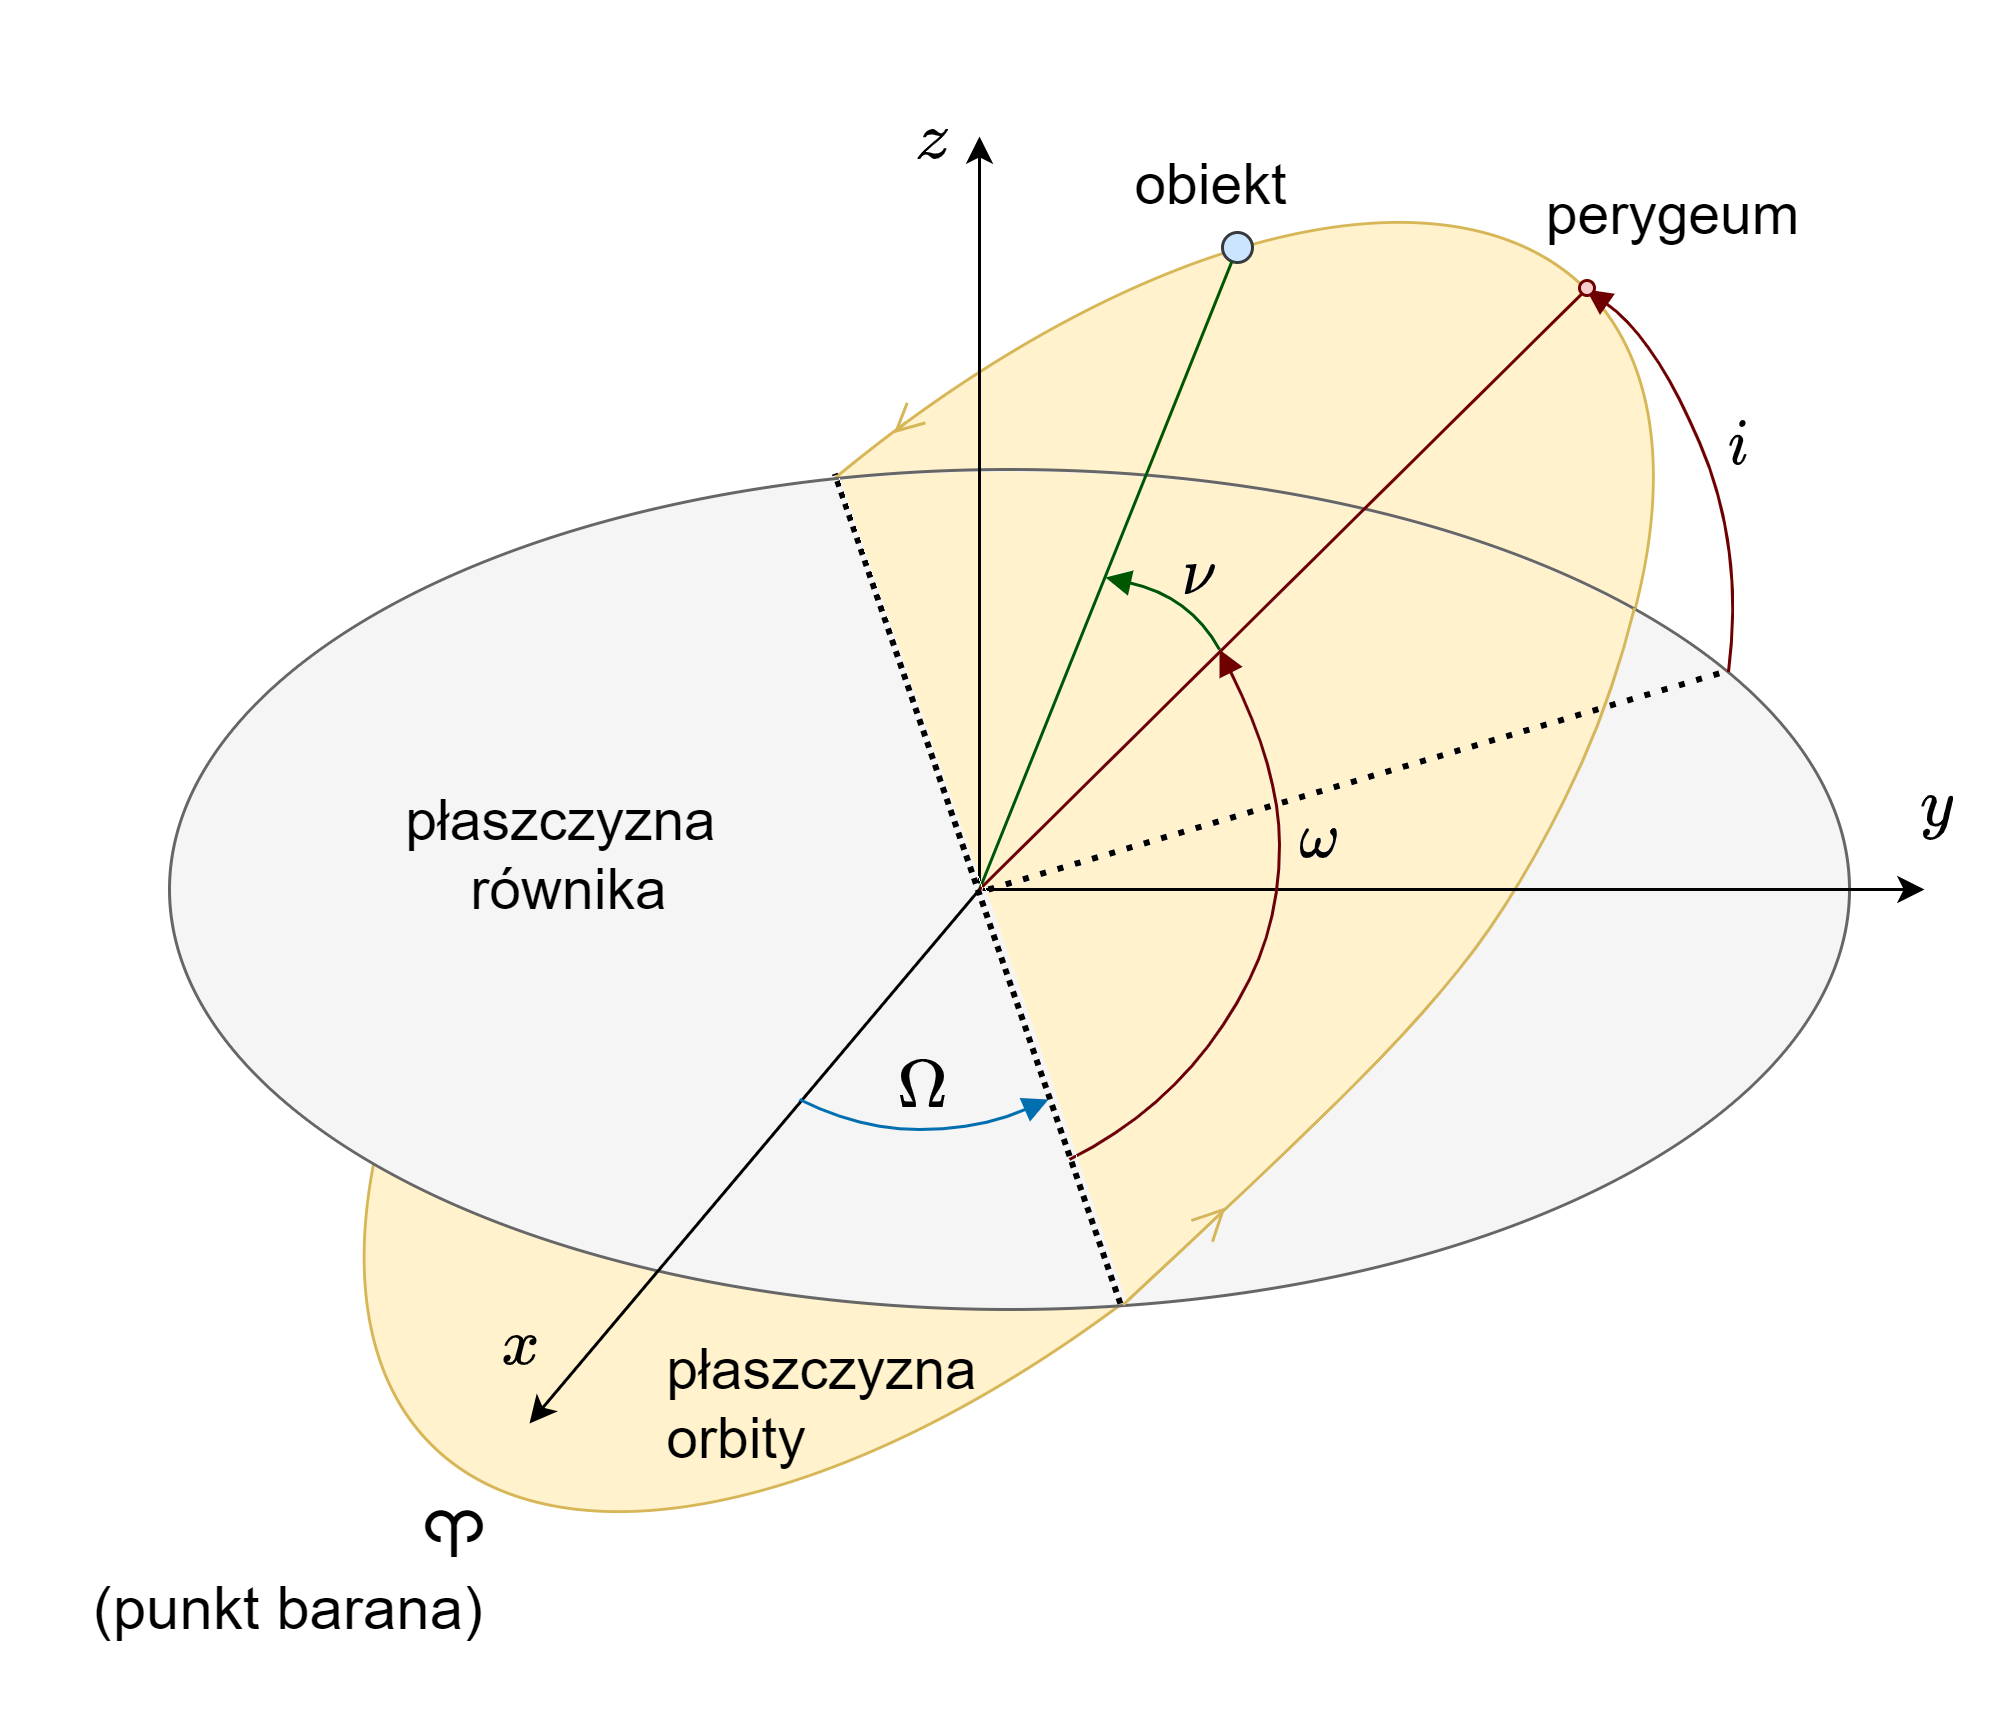
\includegraphics[width=\textwidth]{tex/img/diagramelementy.png}
    \caption{Układ referencyjny ECI oraz część elementów orbitalnych: inklinacja $i$, długość węzła wstępującego $\Omega$, argument perygeum $\omega$ i anomalia prawdziwa $\nu$}
    \label{fig:elementy-szkic}
    \end{figure}


\subsection{Transformacja wektora stanu na elementy orbitalne}
Dysponując wektorem stanu (wektor położenia $\mathbf{r}$ i wektor prędkości $\mathbf{v}$ w układzie ECI) można wyznaczyć elementy orbitalne. Potrzebny jest też powiązany z prawem powszechnego ciążenia standardowy parametr grawitacyjny $\mu$, będący iloczynem stałej grawitacyjnej i sumy mas ciała orbitującego i centralnego.
\begin{equation}
\mu = G(M+m) \stackrel{M >> m}{\approx} GM
\end{equation}

Procedura wyznaczenia elementów orbitalnych z wektora stanu: \newline
Wyznaczenie momentu pędu:
\begin{equation}
\mathbf{h} = \mathbf{r} \times \mathbf{v}
\end{equation}
 Wyznaczenie inklinacji:
\begin{equation}
i = \cos^{-1}{\left(\frac{h_z}{\|\mathbf{h}\|}\right)}
\end{equation}
 Wyznaczenie: osi apsyd i długości węzła wstępującego:
\begin{align}
\mathbf{N} &= [0,0,1] \times \mathbf{h} \\
\Omega &= \cos^{-1}{\left(\frac{N_x}{\|\mathbf{N}\|}\right)}
\end{align}
 Wyznaczenie mimośrodu:
\begin{equation}
\mathbf{e} = \frac{1}{\mu}\left(\mathbf{v}\times\mathbf{h}-\mu\frac{\mathbf{r}}{\|\mathbf{r}\|}\right) 
\end{equation}
\begin{equation}
e = \|\mathbf{e}\|
\end{equation}
 Wyznaczenie argumentu perygeum:
\begin{equation}
\omega = cos^{-1}\left(\frac{\mathbf{N}\cdot\mathbf{e}}{\|\mathbf{N}\|\|\mathbf{e}\|}\right)
\end{equation}
Jeśli $e_Z$ < 0:
\begin{equation}
\omega = 360\degree - \omega
\end{equation}
 Wyznaczenie anomalii prawdziwej:
\begin{equation}
\theta = cos^{-1}\left(\frac{\mathbf{e}\cdot\mathbf{r}}{\|\mathbf{e}\|\|\mathbf{r}\|}\right)
\end{equation}
Jeśli $\mathbf{r} \cdot \mathbf{v}  < 0$:
\begin{equation}
\theta = 360\degree - \theta
\end{equation}
 Wyznaczenie półosi wielkiej:
\begin{equation}
r_p = \frac{h^2}{\mu}\frac{1}{1+\|\mathbf{e}\| \cos(0\degree)}
\end{equation}
\begin{equation}
r_a = \frac{h^2}{\mu}\frac{1}{1+\|\mathbf{e}\| \cos(180\degree)}
\end{equation}
\begin{equation}
a = \frac{r_p + r_a}{2}
\end{equation}

\subsection{Metoda Gaussa}
Metoda Gaussa pozwala na wyznaczenie wektora stanu obiektu na podstawie trzech obserwacji \cite{Curtis2013}. Wymaga to pomiaru składającego się z się z czasu pomiaru $t_i$, wektora położenia obserwatora $R_i$ oraz wersora kierunkowego obserwacji $\hat{\rho_i}$. Wersor kierunkowy można wyznaczyć na podstawie zaobserwowanych współrzędnych astronomicznych  \cite{Astronomiczne}. Schemat obserwacji pokazuje Rysunek. \ref{fig:obserwacja}.

    \begin{figure}[h]
    \centering
    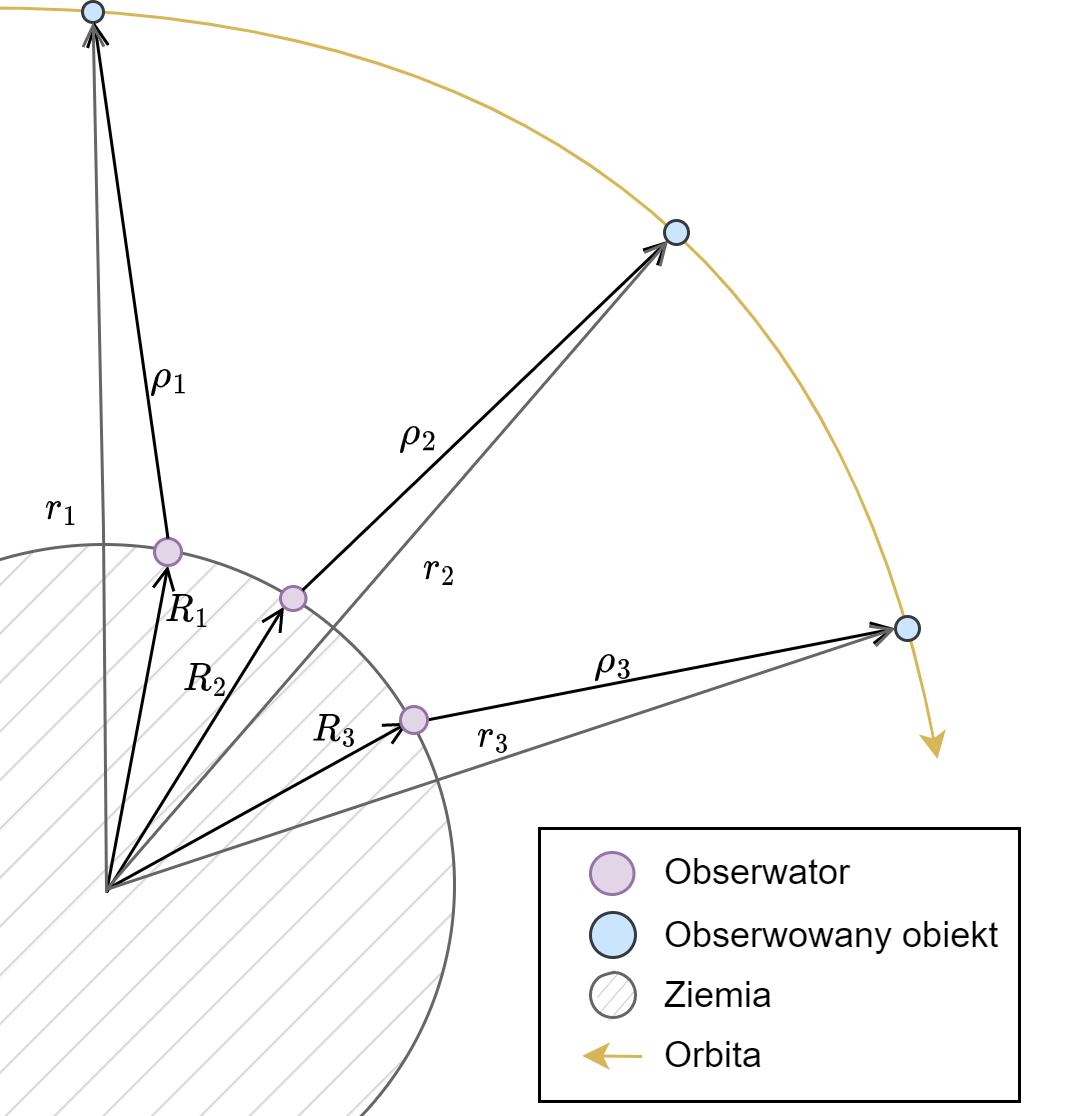
\includegraphics[width=0.8\textwidth]{tex/img/ziemia-orbita.png}
    \caption{Schemat wektorów używanych do wyznaczenia orbity metodą Gaussa}
    \label{fig:obserwacja}
    \end{figure}


Kolejne kroki metody to: \newline
Wyznaczenie międzyczasów:
\begin{align}
\tau_1 &= t_1 - t_2 \\
\tau &= t_3 - t_1 \\
\tau_3 &= t_3 - t_2 
\end{align}
Wyznaczenie iloczynów: 
\begin{align}
\mathbf{p}_1 &= \mathbf{\hat{\boldsymbol\rho}}_2 \times  \mathbf{\hat{\boldsymbol\rho}}_3 \\
\mathbf{p}_2 &= \mathbf{\hat{\boldsymbol\rho}}_1 \times  \mathbf{\hat{\boldsymbol\rho}}_3\\
\mathbf{p}_3 &= \mathbf{\hat{\boldsymbol\rho}}_1 \times  \mathbf{\hat{\boldsymbol\rho}}_2\\
D_0 &= \hat{\boldsymbol\rho}_1 \cdot \mathbf{p}_1
\end{align}
Wyznaczenie macierzy $\boldsymbol{D}_{3x3}$:
\begin{equation}
D_{ij} = \boldsymbol R_i \cdot \boldsymbol p_j
\end{equation}
Wyznaczenie współczynników A i B:
\begin{align}
A &= \frac{1}{D_0} \left(-D_{12}\frac{\tau_3}{\tau}+D_{22}+D_{32}\frac{\tau_1}{\tau}\right) \\
B &= \frac{1}{6D_0} \left(D_{12}(\tau_3^2-\tau^2)\frac{\tau_3}{\tau}+D_{32}(\tau^2-\tau^2_1)\frac{\tau_1}{\tau}\right)
\end{align}
Wyznaczenie współczynnika E: 
\begin{equation}
E = \mathbf{R}_2 \cdot \boldsymbol{\hat{\rho}}_2
\end{equation}
Wyznaczenie współczynników a, b i c:
\begin{align}
a &= -(A^2+2AE+\|\mathbf{R}_2\|^2)\\
b &= -2\mu B(A+E)\\
c &=  -\mu^2B^2 
\end{align}
Wyznaczenie rzeczywistego, nieujemnego pierwiastka wielomianu i przyjęcie go jako wartość $\|\boldsymbol{r}_2\|$:
\begin{equation}
x^8 + ax^6 + bx^3 + c = 0
\end{equation}
Wyznaczenie wartości wektora obserwacji:
\begin{align}
\|\boldsymbol\rho_2\| &= A + \frac{\mu B}{\|\mathbf{r}_2\|^3} \\
\|\boldsymbol\rho_1\| &= \frac{1}{D_0} \left(\frac{6\left(D_{31}\frac{\tau_1}{\tau_3}+D_{21}\frac{\tau}{\tau_3}\right)\|\mathbf{r}_2\|^3 + \mu D_{31} (\tau^2-\tau_1^2)\frac{\tau_1}{\tau_3}}
{6\|\mathbf{r}_2\|^3+\mu(\tau^2-\tau^2_3)}   -D_{11} \right) \\
\|\boldsymbol\rho_3\| &= \frac{1}{D_0} \left(\frac{6\left(D_{13}\frac{\tau_3}{\tau_1}+D_{23}\frac{\tau}{\tau_1}\right)\|\mathbf{r}_2\|^3 + \mu D_{13} (\tau^2-\tau_3^2)\frac{\tau_3}{\tau_1}}
{6\|\mathbf{r}_2\|^3+\mu(\tau^2-\tau^2_3)}  -D_{33}  \right) \\
\end{align}
Wyznaczenie wektora położenia:
\begin{align}
\mathbf{r}_1 &= \mathbf{R}_1 + \|\boldsymbol{\rho}_1\| \boldsymbol{\hat{\rho}}_1 \\
\mathbf{r}_2 &= \mathbf{R}_2 + \|\boldsymbol{\rho}_2\| \boldsymbol{\hat{\rho}}_2 \\
\mathbf{r}_3 &= \mathbf{R}_3 + \|\boldsymbol{\rho}_3\| \boldsymbol{\hat{\rho}}_3
\end{align}
Wyznaczenie współczynników Lagrange'a
\begin{align}
f_1 &= 1 - \frac{1}{2}\frac{\mu}{\|\mathbf{r}_2\|^3}\tau_1^2 \\
f_3 &= 1 - \frac{1}{2}\frac{\mu}{\|\mathbf{r}_2\|^3}\tau_3^2 \\
f_1 &= \tau_1 - \frac{1}{6}\frac{\mu}{\|\mathbf{r}_2\|^3}\tau_1^3 \\
g_3 &= \tau_3 - \frac{1}{6}\frac{\mu}{\|\mathbf{r}_2\|^3}\tau_3^3 \\
\end{align}
Wyznaczenie wektora prędkości:
\begin{equation}
\mathbf{v}_2 = \frac{1}{f_1g_3-f_3g_1}\left(-f_3\mathbf{r_1}+f_1\mathbf{r_3}\right)
\end{equation}

         % Wygodnie jest trzymać każdy rozdział w osobnym pliku.
\clearpage % Rozdziały zaczynamy od nowej strony.
\section{Cel i zakres projektu}

Celem pracy było wykorzystanie wybranej metody wyznaczania orbity statku kosmicznego na podstawie obserwacji naziemnych. Zaimplementowano metodę Gaussa wraz z poprawką iteracyjną. Do sprawdzenia poprawności działania metody stworzono generator obserwacji, który na podstawie modelu keplerowskiego i założonych elementów orbitalnych wyznacza dane obserwacyjne. Wykonano również walidację korzystając z danych wygenerowanych przy pomocy zewnętrznego programu do symulacji nocnego nieba Stellarium \cite{Stellarium}.

\clearpage % Rozdziały zaczynamy od nowej strony.
\section{Walidacja działania metody}

Do wygenerowania danych użyto informacji z TLE (Two Line Element) Międzynarodowej Stacji Kosmicznej z 19 grudnia 2022, pobranych ze strony archiwizującej informacje o satelitach CelesTrak \cite{Celestrak}:
\begin{verbatim}
1 25544U 98067A   22353.42711160  .00011227  00000-0  20403-3 0  9992
2 25544  51.6432 138.9346 0003592 174.7295 234.7524 15.50052736373915
\end{verbatim}

Format TLE nie zawiera informacji o elementach orbitalnych zdefiniowanych tak jak w rozdziale \ref{ch:wektory-stanu}. Zamiast półosi wielkiej podaje dodatkowe informacje takie jak średnia częstość kołowa, jej pierwszą i drugą pochodną, współczynnik ciśnienia promieniowania, anomalię średnią oraz informacje o obiekcie i orbicie \cite{TLE}.

Półoś wielką można wyznaczyć na podstawie częstości kołowej zgodnie ze wzorem:
\begin{equation}
a = \frac{\mu^{\frac{1}{3}}}{\left(\frac{2\pi}{24\cdot60\cdot60}n\right)^{\frac{2}{3}}}
\end{equation}
Gdzie: 
\begin{itemize}
\item n -- częstość kołowa [obr/dzień]
\item       $\mu$ -- $GM$ standardowy parametr grawitacyjny dla Ziemi
\end{itemize}

Na podstawie danych TLE uzyskano klasyczne elementy orbitalne. Następnie wygenerowano trzy zestawy danych obserwacyjnych i wykonano 5 porównań:
\begin{itemize}
    \item trzy obserwacje w pobliżu górowania, o niewielkich różnicach czasu między obserwacjami 
    \item trzy obserwacje dokonane podczas wschodu, górowania i zachodu obserwowanego obiektu
    \item powyższe dwa przypadki z symulowanym błędem pomiaru
    \item sytuacja hipotetyczna - obserwacje równomiernie oddzielone na całej orbicie
    \item obserwacje dokonane w symulatorze nocnego nieba Stellarium
\end{itemize}

\subsection{Wspólne stałe}
Podczas wszystkich porównań przyjęto następujące wspólne stale:

        \begin{align*}
             \phi &= 51\degree 23'15.49" \\
             H &= 153 m \\
             R_{E} &= 6378 km \\
             f &= 0.003353 \\
             \mu &= 3,986004418 \cdot 10^{14} \frac{m^3}{s^2}
        \end{align*}
    Gdzie:
        \begin{itemize}
            \item  $ \phi$  -- szerokość geograficzna obserwatora 
            \item $H$ -- wysokość nad poziomem morza obserwatora
            \item       $ R_{E}$ -- promień Ziemi  
            \item        $f$ -- spłaszczenie Ziemi 
            \item $\theta$ -- lokalny czas gwiazdowy obserwacji
        \end{itemize}
        
Współrzędne kartezjańskie obserwatora dla każdej obserwacji wyznaczono ze wzoru:

            \begin{center}
            \begin{equation}
              \begin{split}
              \mathbf{R} & =\left[ \cfrac{R_e}{\sqrt{1-(2f-f^2)sin^2\phi}} + H\right]\cdot \cos{\phi}(\cos{{\theta}\hat{I}+\sin{\theta}\hat{J}}) \\
            &+  \left[ \cfrac{R_e(1-f)^2}{\sqrt{1-(2f-f^2)sin^2\phi}} + H\right] \cdot \sin{\phi} 
            \end{split}
            \end{equation}
        \end{center}



\FloatBarrier
\subsection{Obserwacja w pobliżu górowania}
\label{sub:Krotki}
      \subsubsection{Dane obserwacyjne}

    Czas obserwacji odpowiada zmianie anomalii o kąt 10\degree: 
        \begin{align*}
            t_{1} &= 0 s \\
            t_{2} &= 77 s  \\
            t_{3} &= 154 s
        \end{align*}    
        
    Czas gwiazdowy obserwacji: 
        \begin{align*}
            \theta_1 &= 301.7692\degree \\
            \theta_2 &= 302.0933\degree  \\
            \theta_3 &= 302.4175\degree
        \end{align*}

    Wykorzystane pozycje [km]: 
   
            \begin{center}
              $\begin{bmatrix}
                R_{1x} & R_{1y} & R_{1z} \\
                R_{2x} & R_{2y} & R_{2z} \\
                R_{3x} & R_{3y} & R_{3z} 
            \end{bmatrix}
            =
            \begin{bmatrix}
                338 & -5050 & 4530 \\
                843 & -5216 & 4269 \\
                1342 & -5342 & 3975
            \end{bmatrix}    $
        \end{center}

    \subsubsection{Wyniki}
    
    Wszystkie błędy są mniejsze niż 1e-06. Jest to zgodne z oczekiwaniami, ponieważ model obserwacyjny i metoda wyznaczania korzystają z idealnego modelu keplerowskiego.

    \begin{table}[!ht]  \centering
    \caption{Krótki czas między obserwacjami - porównanie wyników}
    \label{tab:Krotki-table}
    \begin{tabular} {| l | r | r | r |} \hline
        Parametr 1          & Wartość referencyjna  & Wartość wyznaczona  & Błąd \\ \hline\hline
        Moduł położenia w 2 pozycji     & 6793 km    & 6793 km        & 1e-09 km\\ \hline
        Moduł prędkości w 2 pozycji     & 7.7 km/s     & 7.7 km/s     & 5e-11 km/s\\ \hline
        Mimośród                        & 3.6e-04       & 3.6e-04      & 2e-12 \\ \hline
        Półoś wielka                    & 6794 km    & 6794 km        & 2e-08 \\ \hline
        Inklinacja                      & 51.64\degree & 51.64\degree & 3e-11\degree \\ \hline
        Rektascensja węzła wstępującego & 138.9\degree & 138.9\degree & 4e-11 \degree \\ \hline
        Argument perycentrum            & 174.7\degree & 174.7\degree  & 4e-07 \\ \hline
        Anomalia prawdziwa              & 312\degree   & 312\degree   & 4e-07 \\ \hline
    \end{tabular}
    \end{table}

    \begin{figure}[h]
    \centering
    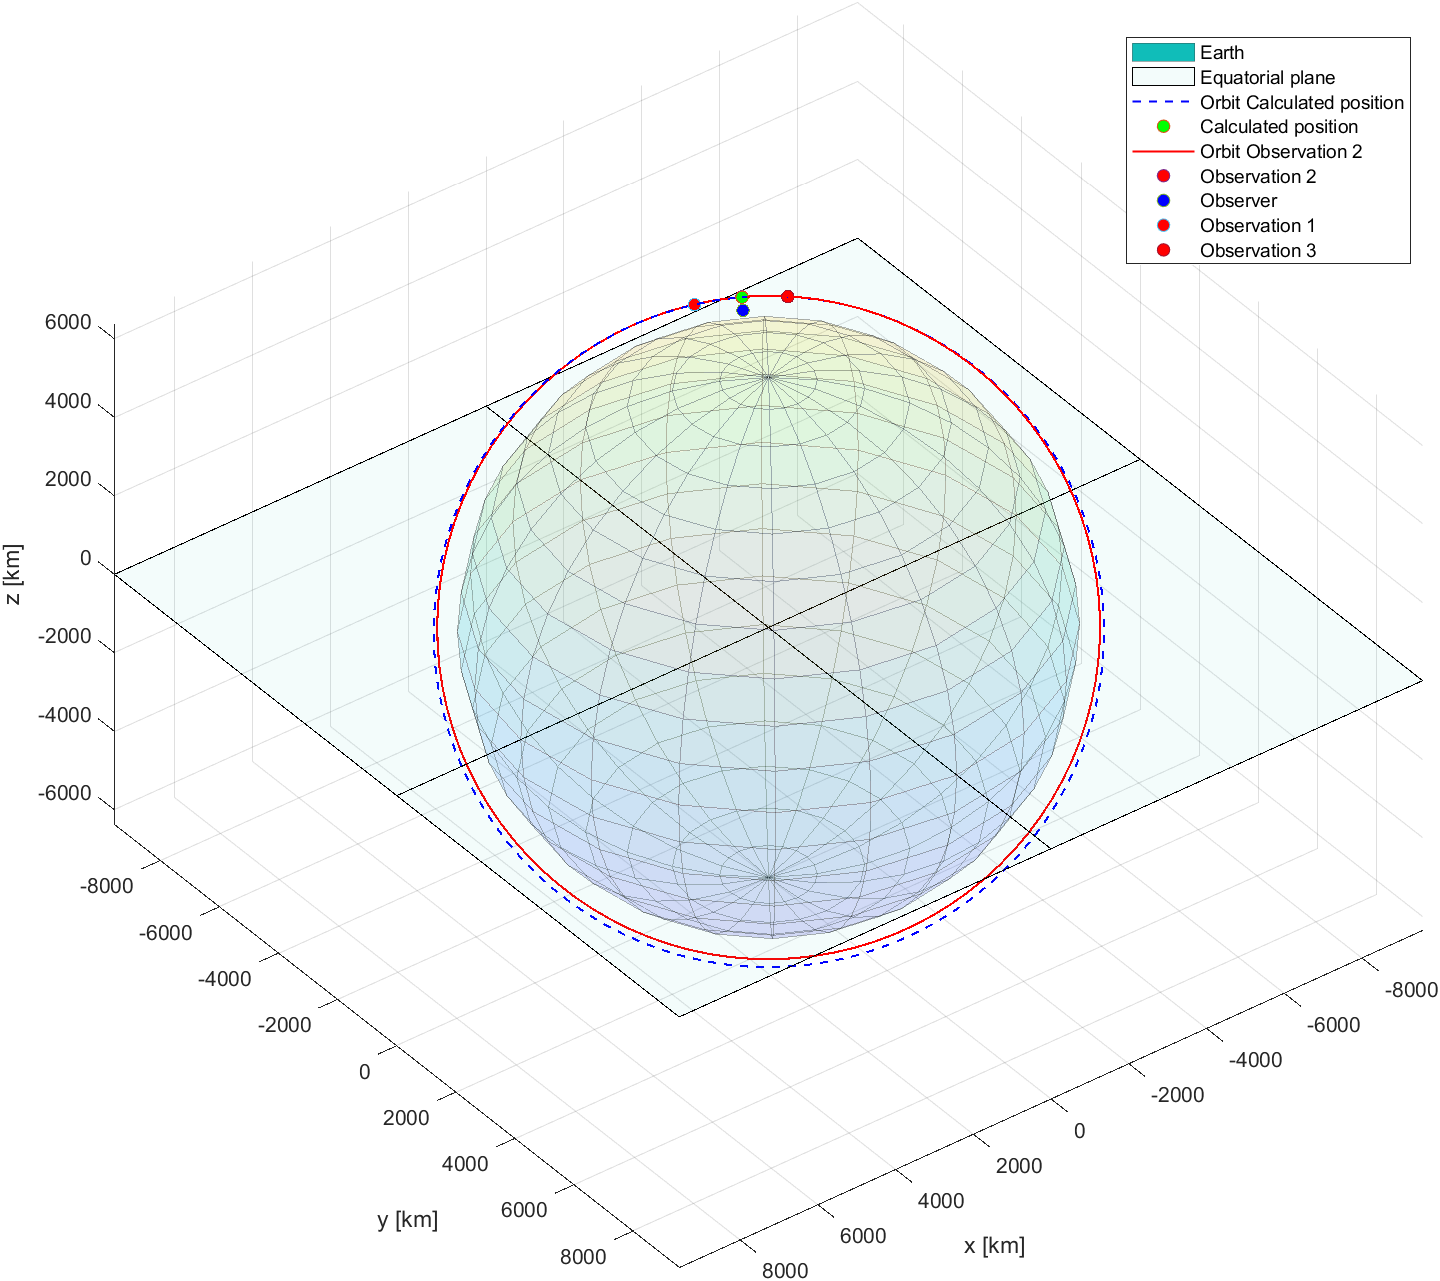
\includegraphics[width=\textwidth]{tex/img/StellariumFigure.png}
    \caption{Krótki czas między obserwacjami - wizualizacja}
    \label{fig:Krotki-1}
    \end{figure}
    
    \begin{figure}[h]
    \centering
    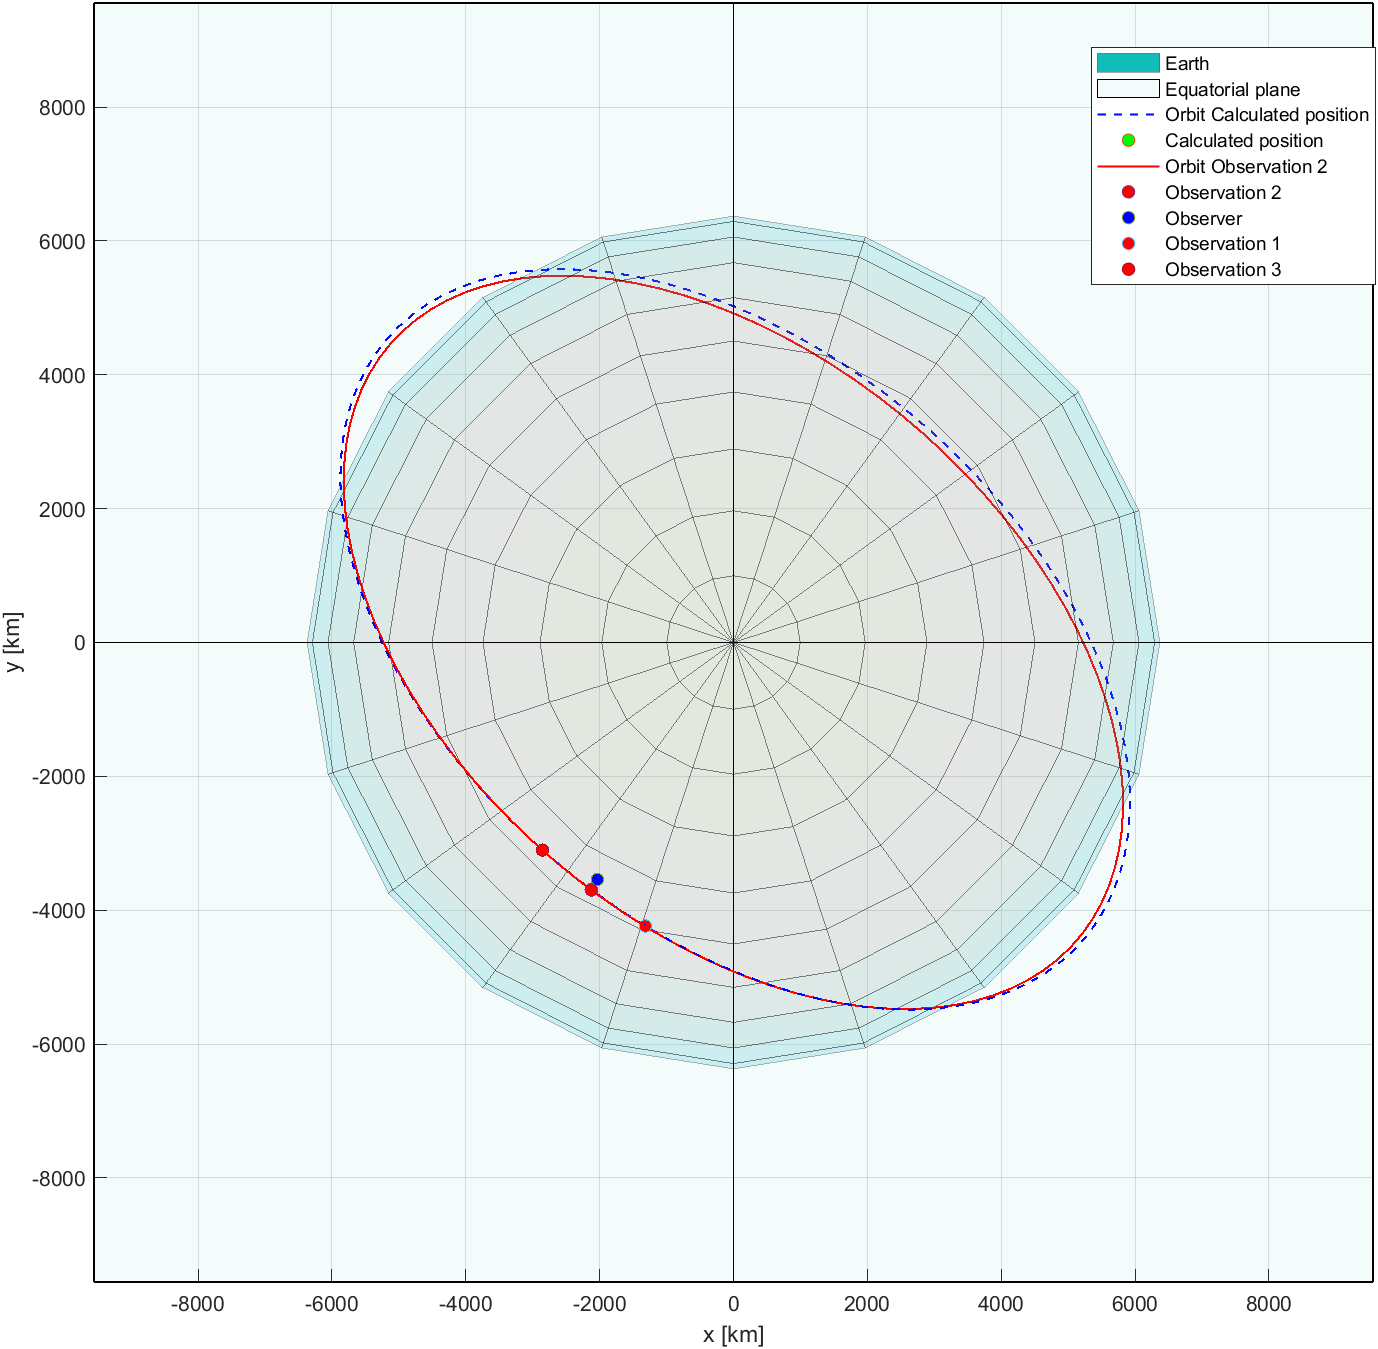
\includegraphics[width=\textwidth]{tex/img/StellariumFigure_rownikowa.png}
    \caption{Krótki czas między obserwacjami - rzut na płaszczyznę równikową}
    \label{fig:Krotki-2}
    \end{figure}


\FloatBarrier
\subsection{Obserwacja podczas pełnego przelotu}
\label{sub:Pelny}
       \subsubsection{Dane obserwacyjne}

    Czas obserwacji odpowiada zmianie anomalii o kąt 30\degree: 
        \begin{align*}
            t_{1} &= 0 s \\
            t_{2} &= 309 s  \\
            t_{3} &= 619 s
        \end{align*}    
        
    Czas gwiazdowy obserwacji: 
        \begin{align*}
            \theta_1 &= 300.7965\degree \\
            \theta_2 &= 302.0933\degree  \\
            \theta_3 &= 303.3900\degree
        \end{align*}

    Wykorzystane pozycje [km]: 
   
            \begin{center}
              $\begin{bmatrix}
                R_{1x} & R_{1y} & R_{1z} \\
                R_{2x} & R_{2y} & R_{2z} \\
                R_{3x} & R_{3y} & R_{3z} 
            \end{bmatrix}
            =
            \begin{bmatrix}
                -1177 & -4328 & 5101 \\
                843 & -5216 & 4269 \\
                2762 & -5474 & 2922
            \end{bmatrix}    $
        \end{center}

    \subsubsection{Wyniki}
    
    Wszystkie błędy są mniejsze niż 1e-06, podobnie jak dla obserwacji o krótkich odstępach między pomiarami.

    \begin{table}[!h] \centering
    \caption{Obserwacje rozproszone - porównanie wyników}
    \label{tab:Dlugi-table}
    \begin{tabular} {| l | r | r | r |} \hline
        Parametr 1          & Wartość referencyjna  & Wartość wyznaczona  & Błąd \\ \hline\hline
        Moduł położenia w 2 pozycji     & 6793 km    & 6793 km        & 1e-09 km\\ \hline
        Moduł prędkości w 2 pozycji     & 7.7 km/s     & 7.7 km/s     & 5e-11 km/s\\ \hline
        Mimośród                        & 3.6e-04       & 3.6e-04      & 1e-11 \\ \hline
        Półoś wielka                    & 6794 km    & 6794 km        & 9e-08 \\ \hline
        Inklinacja                      & 51.64\degree & 51.64\degree & 3e-11\degree \\ \hline
        Rektascensja węzła wstępującego & 138.9\degree & 138.9\degree & 7e-13 \degree \\ \hline
        Argument perycentrum            & 174.7\degree & 174.7\degree  & 1e-06 \\ \hline
        Anomalia prawdziwa              & 312\degree   & 312\degree   & 1e-06 \\ \hline
    \end{tabular}
    \end{table}

    \begin{figure}[h]
    \centering
    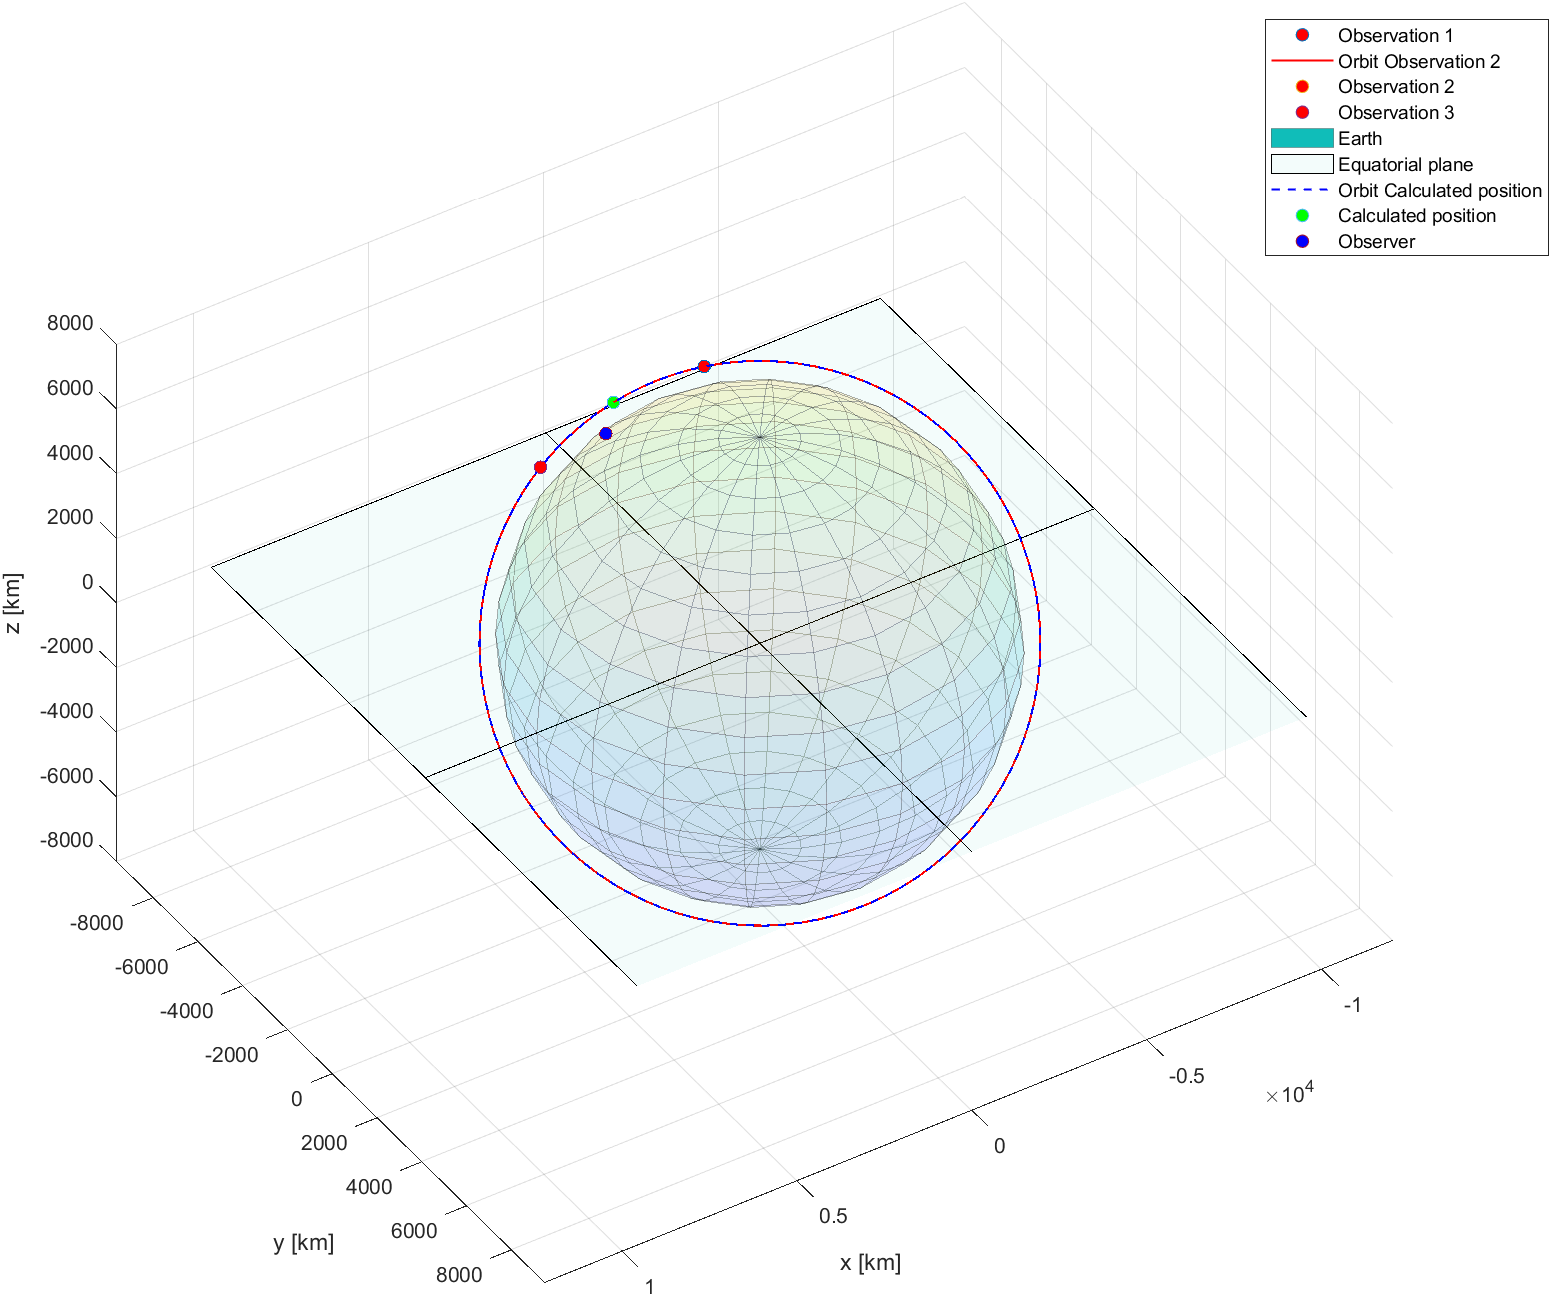
\includegraphics[width=\textwidth]{tex/img/anomaly15.png}
    \caption{Obserwacje rozproszone - wizualizacja}
    \label{fig:Dlugi-1}
    \end{figure}
    
    \begin{figure}[h]
    \centering
    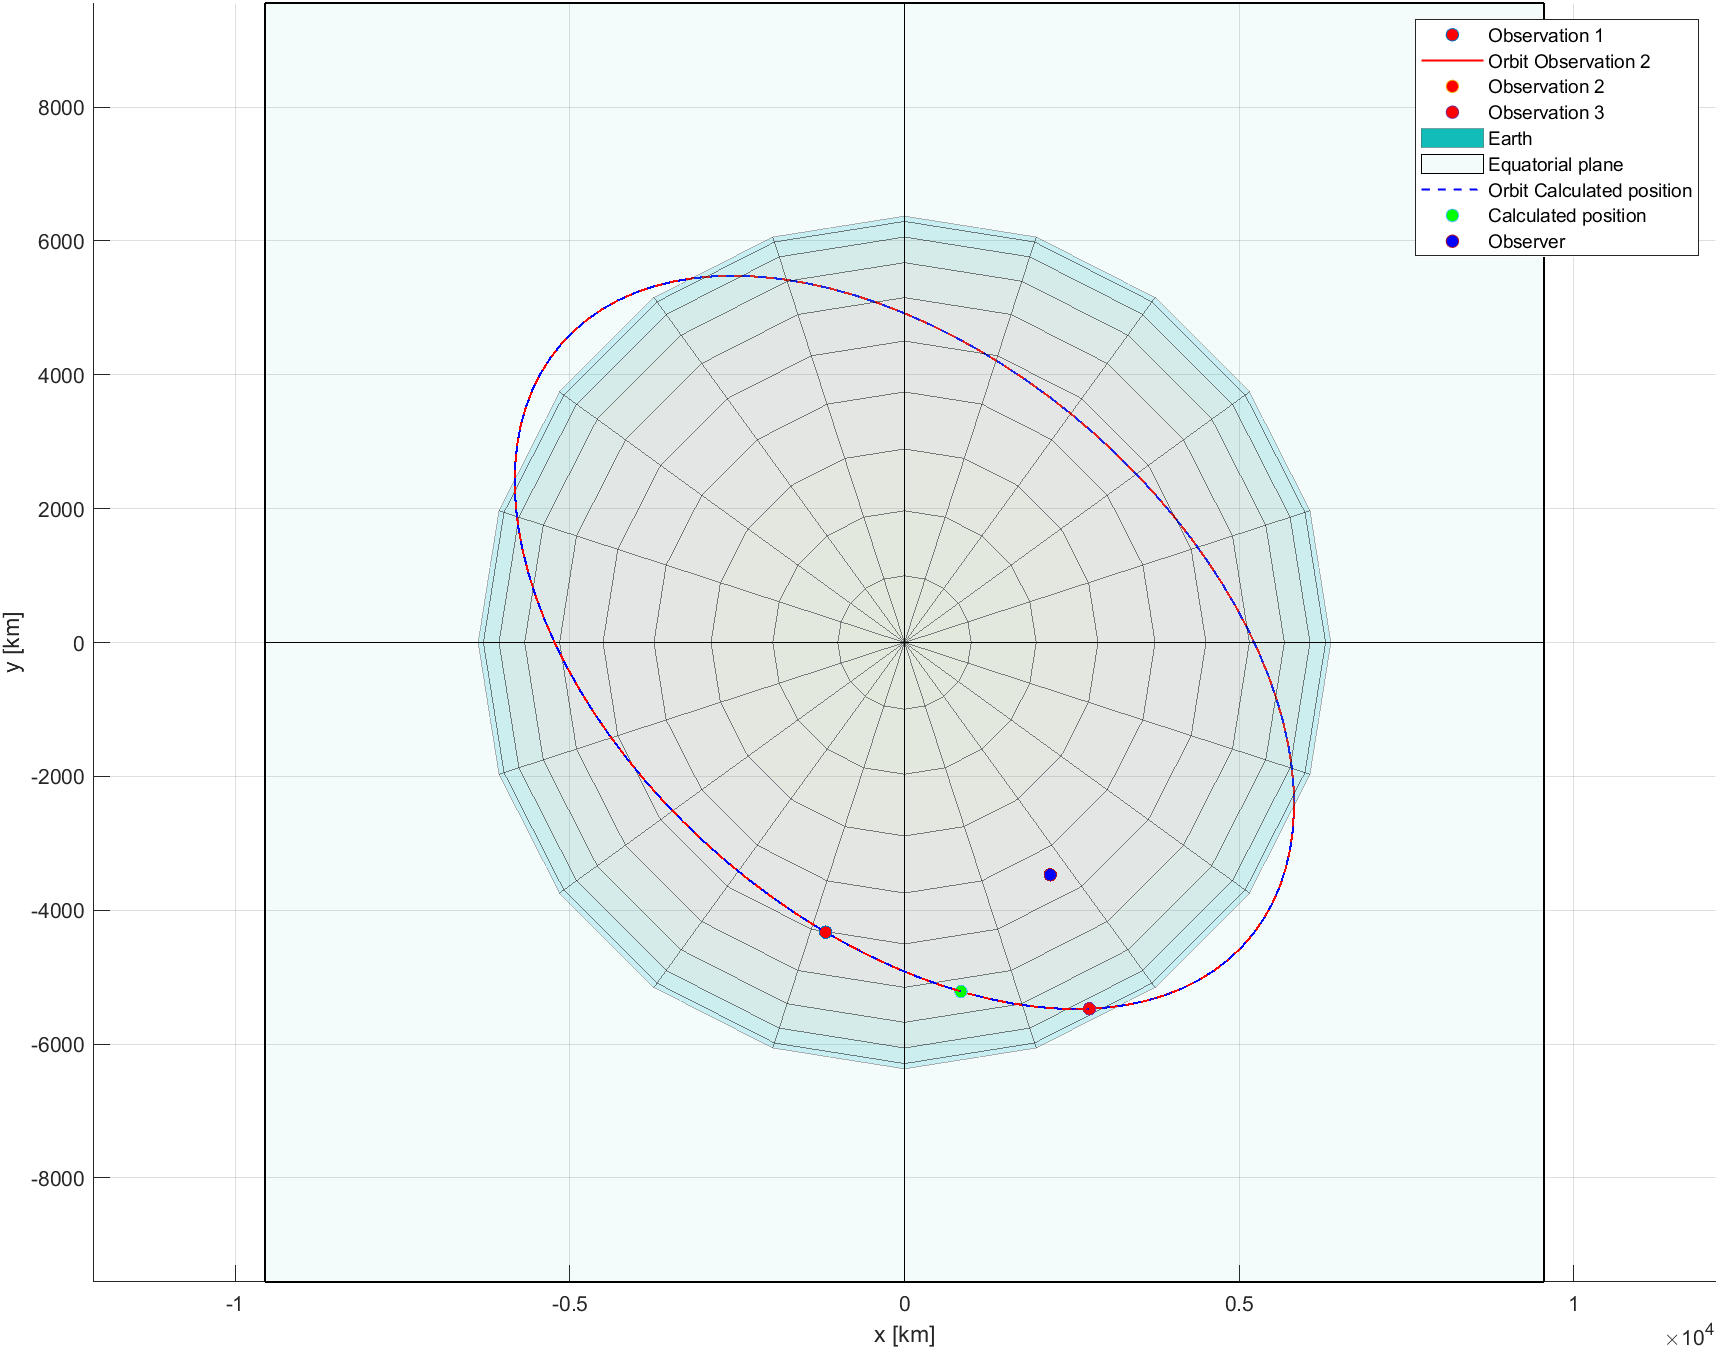
\includegraphics[width=\textwidth]{tex/img/anomaly15_rownikowa.png}
    \caption{Obserwacje rozproszone - rzut na płaszczyznę równikową}
    \label{fig:Dlugi-2}
    \end{figure}



\FloatBarrier
\subsection{Obserwacje zakłócone}

Wyniki uzyskane w podrozdziałach \ref{sub:Krotki} i \ref{sub:Pelny} sugerują, że rozkładanie obserwacji w czasie może nie mieć wpływu na wyniki, ponieważ nawet dla krótkich obserwacji błędy praktycznie nie istnieją. Jest to jednak spowodowane tym, że dane obserwacyjne są generowane w sposób idealny na podstawie idealnego modelu. Poniżej przedstawiono wyniki dla pomiarów nieidealnych.

     \subsubsection{Dane obserwacyjne}
    Takie jak w rozdziałach \ref{sub:Krotki} i \ref{sub:Pelny}. Wersory kierunkowe zaszumiono dodając do każdej współrzędnej losowe liczby z przedziału [0; 0,002] i ponowownie normalizując.
    
    \subsubsection{Wyniki}
    Wyznaczone orbity zostały jakościowo porównane na wykresie \ref{fig:szum_side_by_side}. Zgodnie z oczekiwaniami przeprowadzenie pomiarów z większymi interwałami czasowymi pozwala na wyznaczenie orbity mimo nieidealnych danych.

\begin{figure}%
    \centering
    \subfloat[\centering Krótki czas między obserwacjami]{{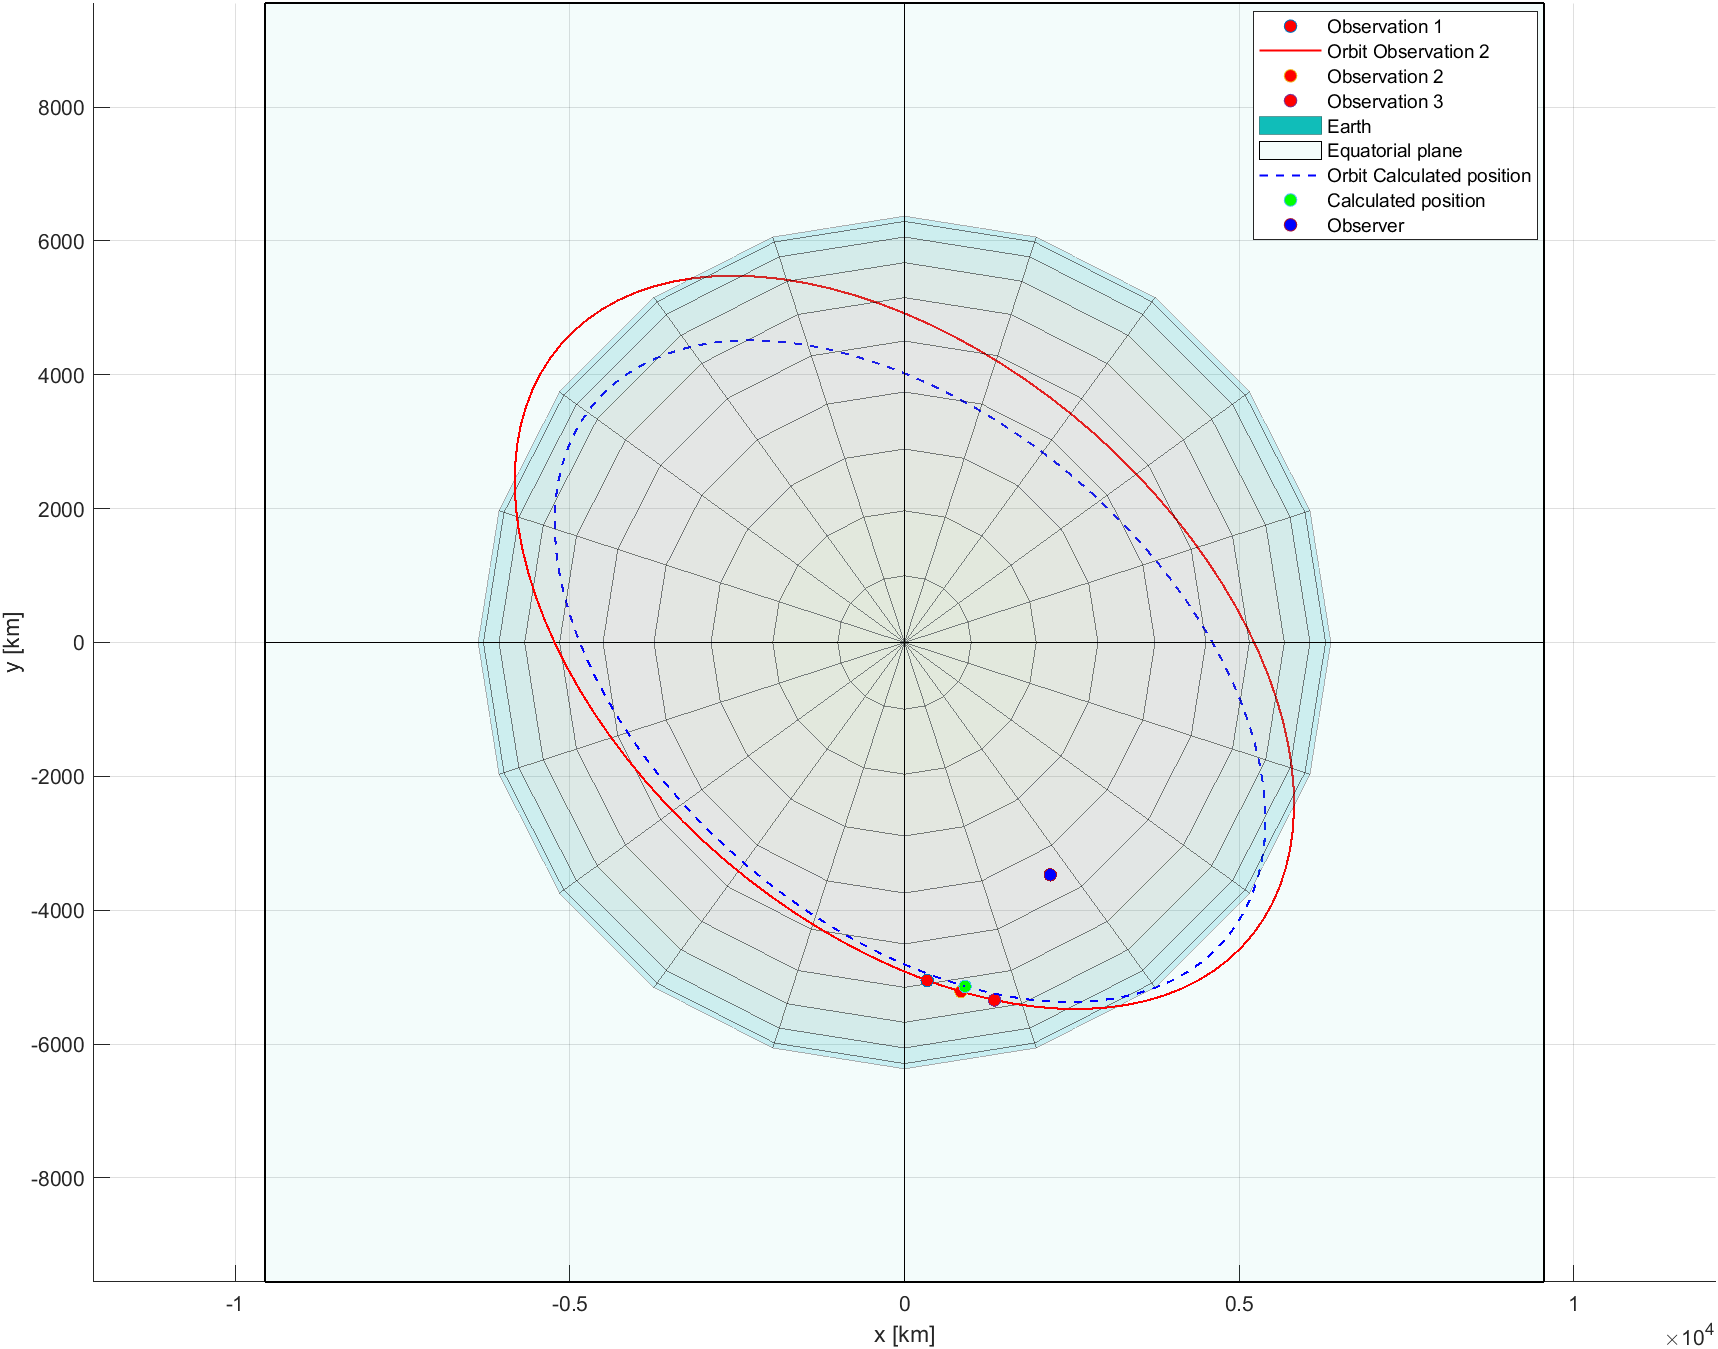
\includegraphics[width=13cm]{tex/img/szum5_rownik.png} }}%
    \qquad
    \subfloat[\centering Obserwacje rozproszone w czasie]{{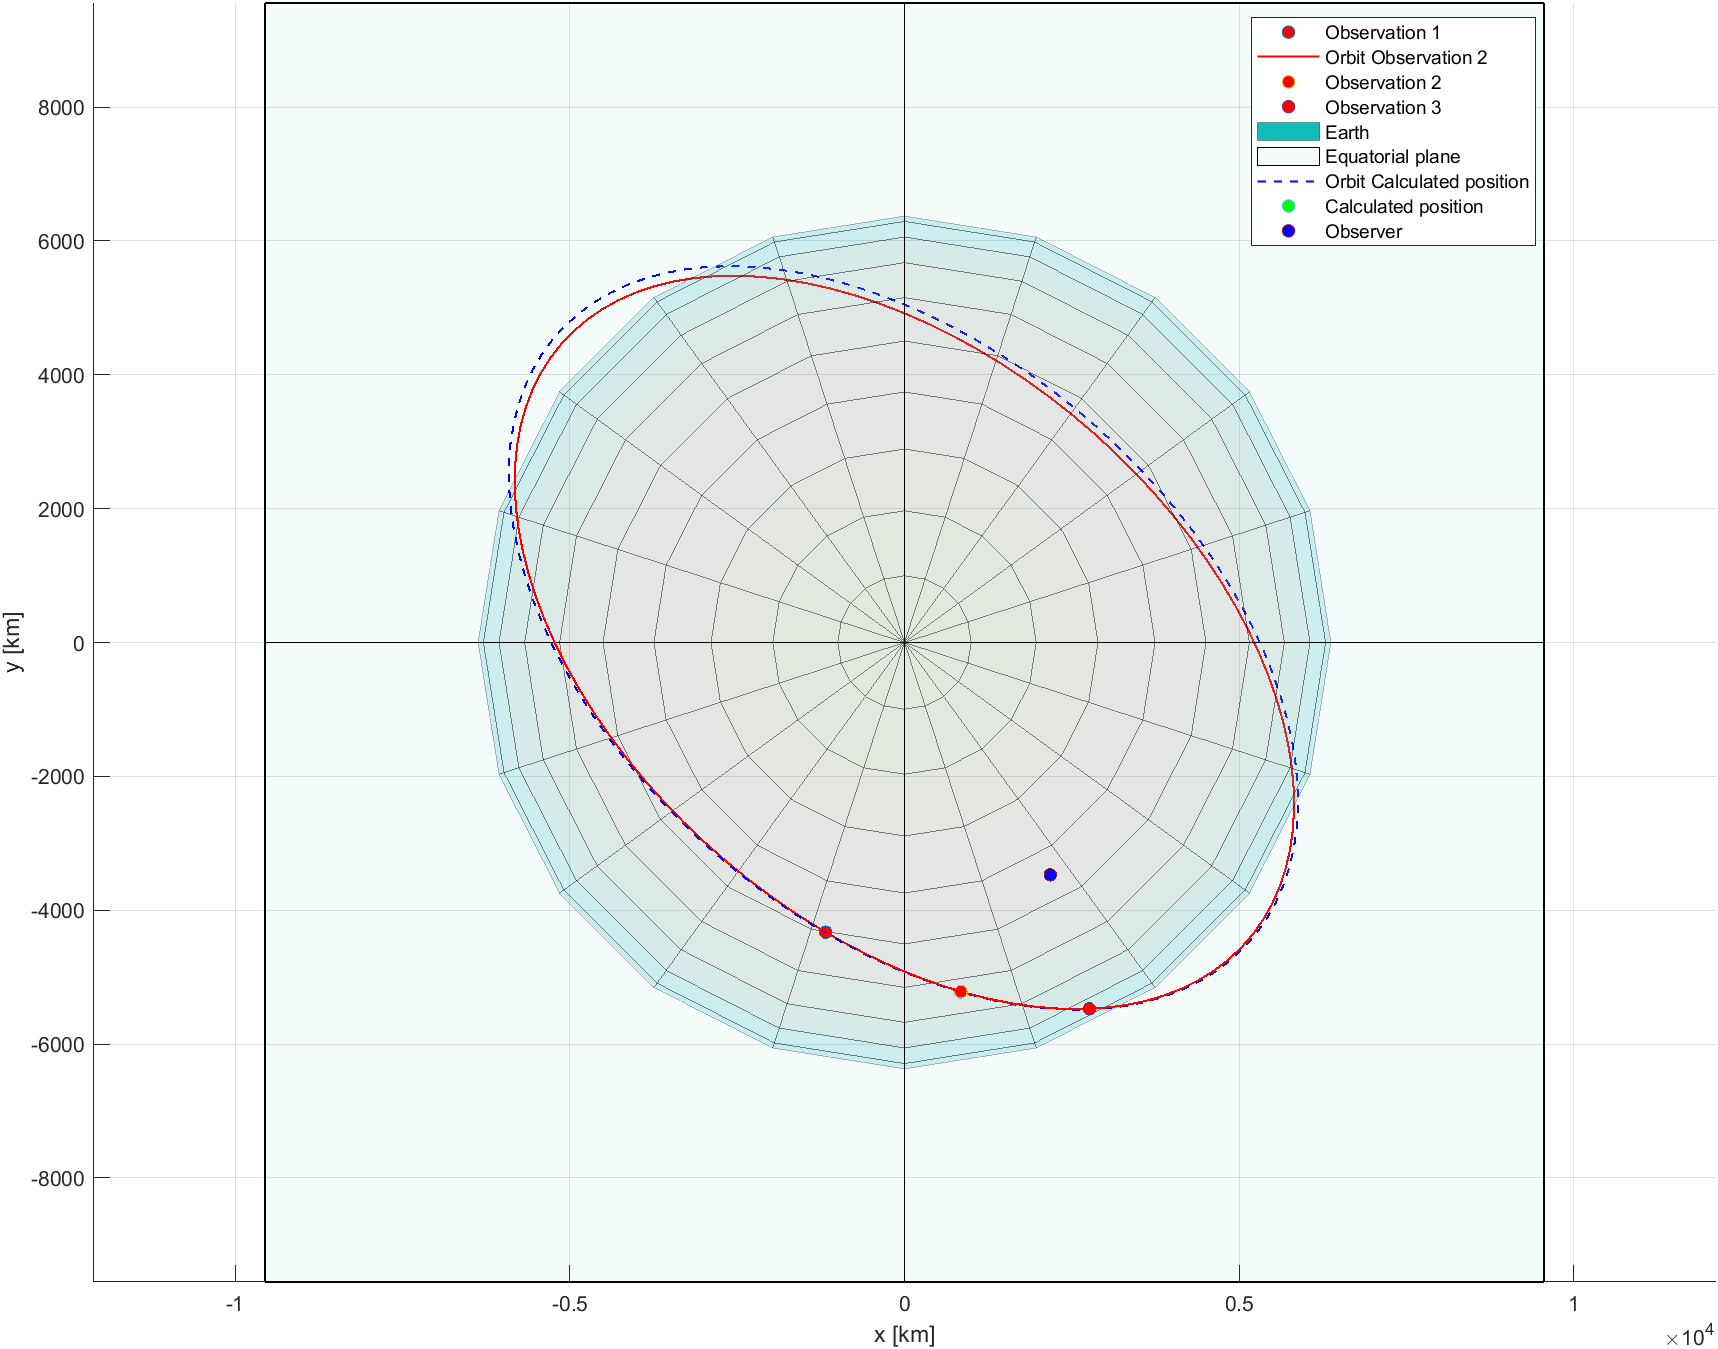
\includegraphics[width=13cm]{tex/img/szum15_rownik.png} }}%
    \caption{Porównanie wpływu dodanego błędu do wersora kierunkowego obserwacji na określoną orbitę w dla dwóch częstości dokonywania pomiarów}%
    \label{fig:szum_side_by_side}%
\end{figure}

\FloatBarrier
\subsection{Obserwacja hipotetyczna}

     \subsubsection{Dane obserwacyjne}

    Czas obserwacji odpowiada zmianie anomalii o kąt 162:\degree: 
        \begin{align*}
            t_{1} &= 0 s \\
            t_{2} &= 1269 s  \\
            t_{3} &= 2538 s
        \end{align*}    
        
    Czas gwiazdowy obserwacji: 
        \begin{align*}
            \theta_1 &= 296.7743\degree \\
            \theta_2 &= 302.0933\degree  \\
            \theta_3 &= 307.4090\degree
        \end{align*}

    Wykorzystane pozycje [km]: 
   
            \begin{center}
              $\begin{bmatrix}
                R_{1x} & R_{1y} & R_{1z} \\
                R_{2x} & R_{2y} & R_{2z} \\
                R_{3x} & R_{3y} & R_{3z} 
            \end{bmatrix}
            =
            \begin{bmatrix}
                -5590 & 934 & 3750 \\
                843 & -5216 & 4269 \\
                5821 & -2385 & -2560
            \end{bmatrix}    $
        \end{center}

    
    \subsubsection{Wyniki}
    Ponieważ wyprowadzenie metody Gaussa wykorzystuje założenie, że czas między pomiarami jest niewielki względem okresu orbity \cite{Curtis2013}, to jest ona nieskuteczna dla długich obserwacji. Zastosowanie poprawki iteracyjnej pozwala na powiększenie zakresu stosowalności, ale ostatecznie i ona zawodzi, gdy metoda podstawowa przestaje generować wystarczająco zbliżone wyniki. Dla przeprowadzonych symulacji maksymalna zmiana anomalii prawdziwej, dla których metoda zwracała poprawne wyniki, wynosiła 160\degree. 

    \begin{figure}[h]
    \centering
    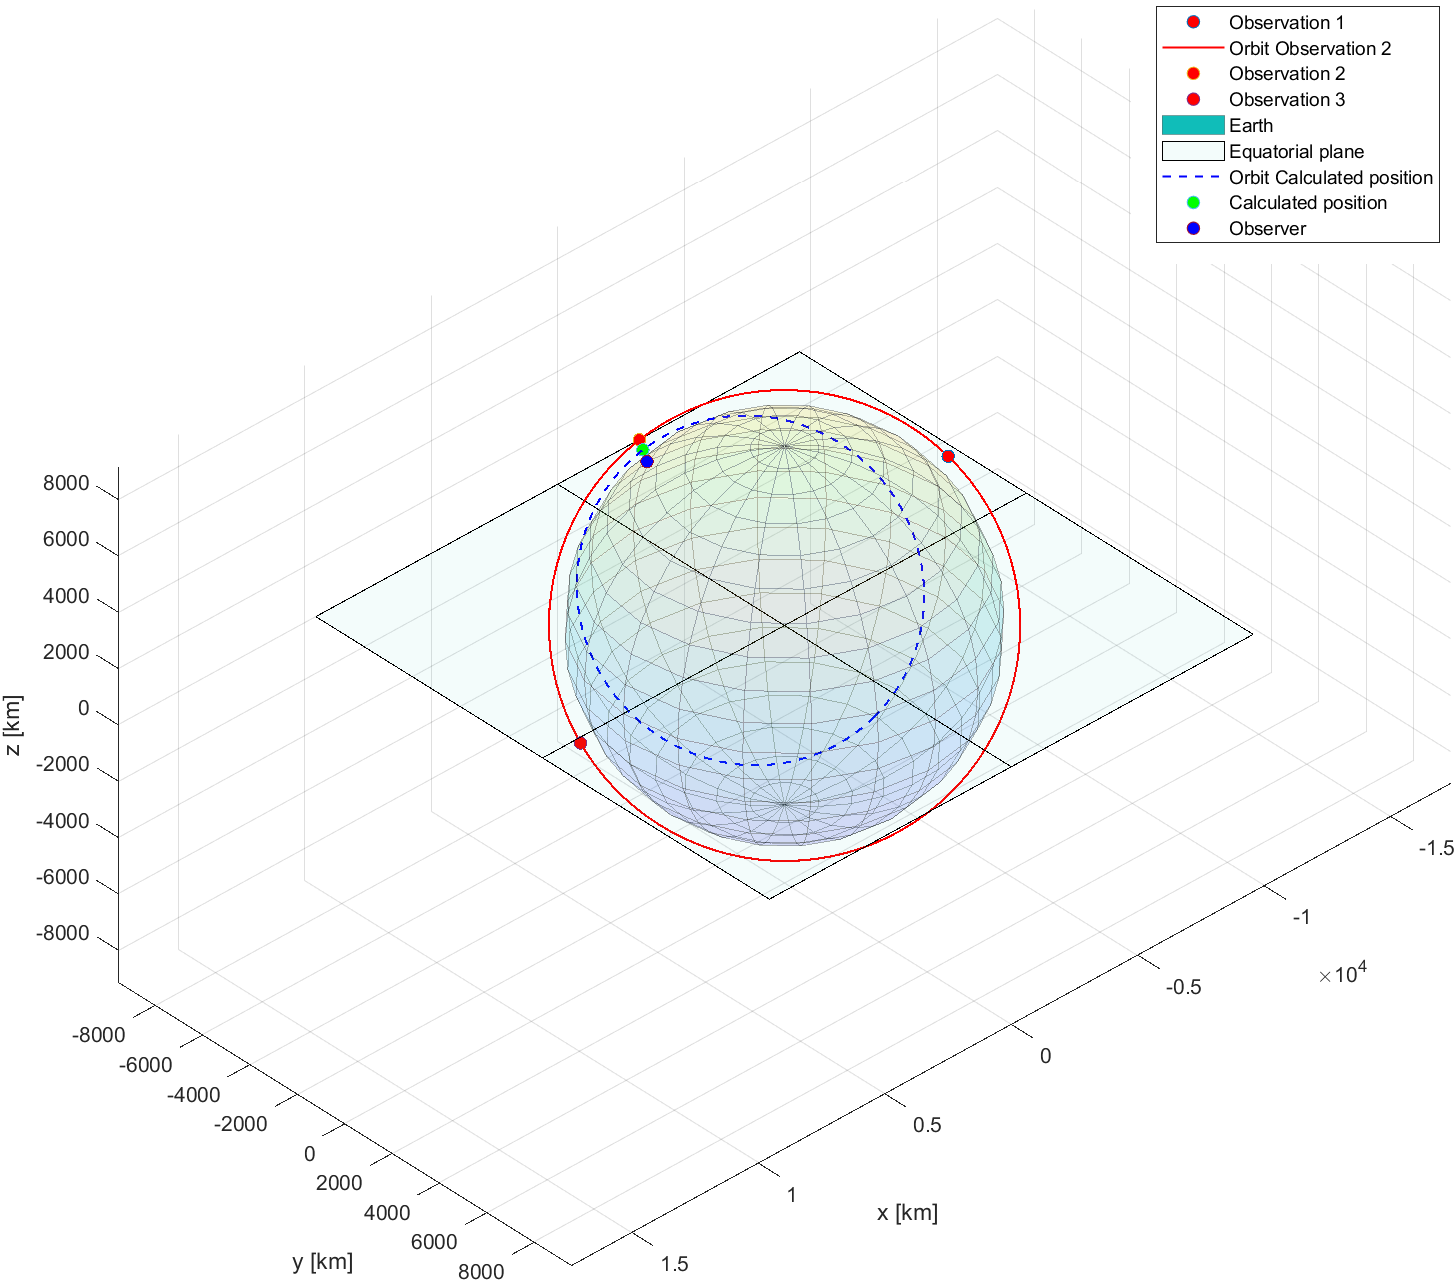
\includegraphics[width=\textwidth]{tex/img/anomaly82.png}
    \caption{Obserwacje hipotetyczne - wizualizacja}
    \label{fig:hipotetyczne-1}
    \end{figure}
    
    \begin{figure}[h]
    \centering
    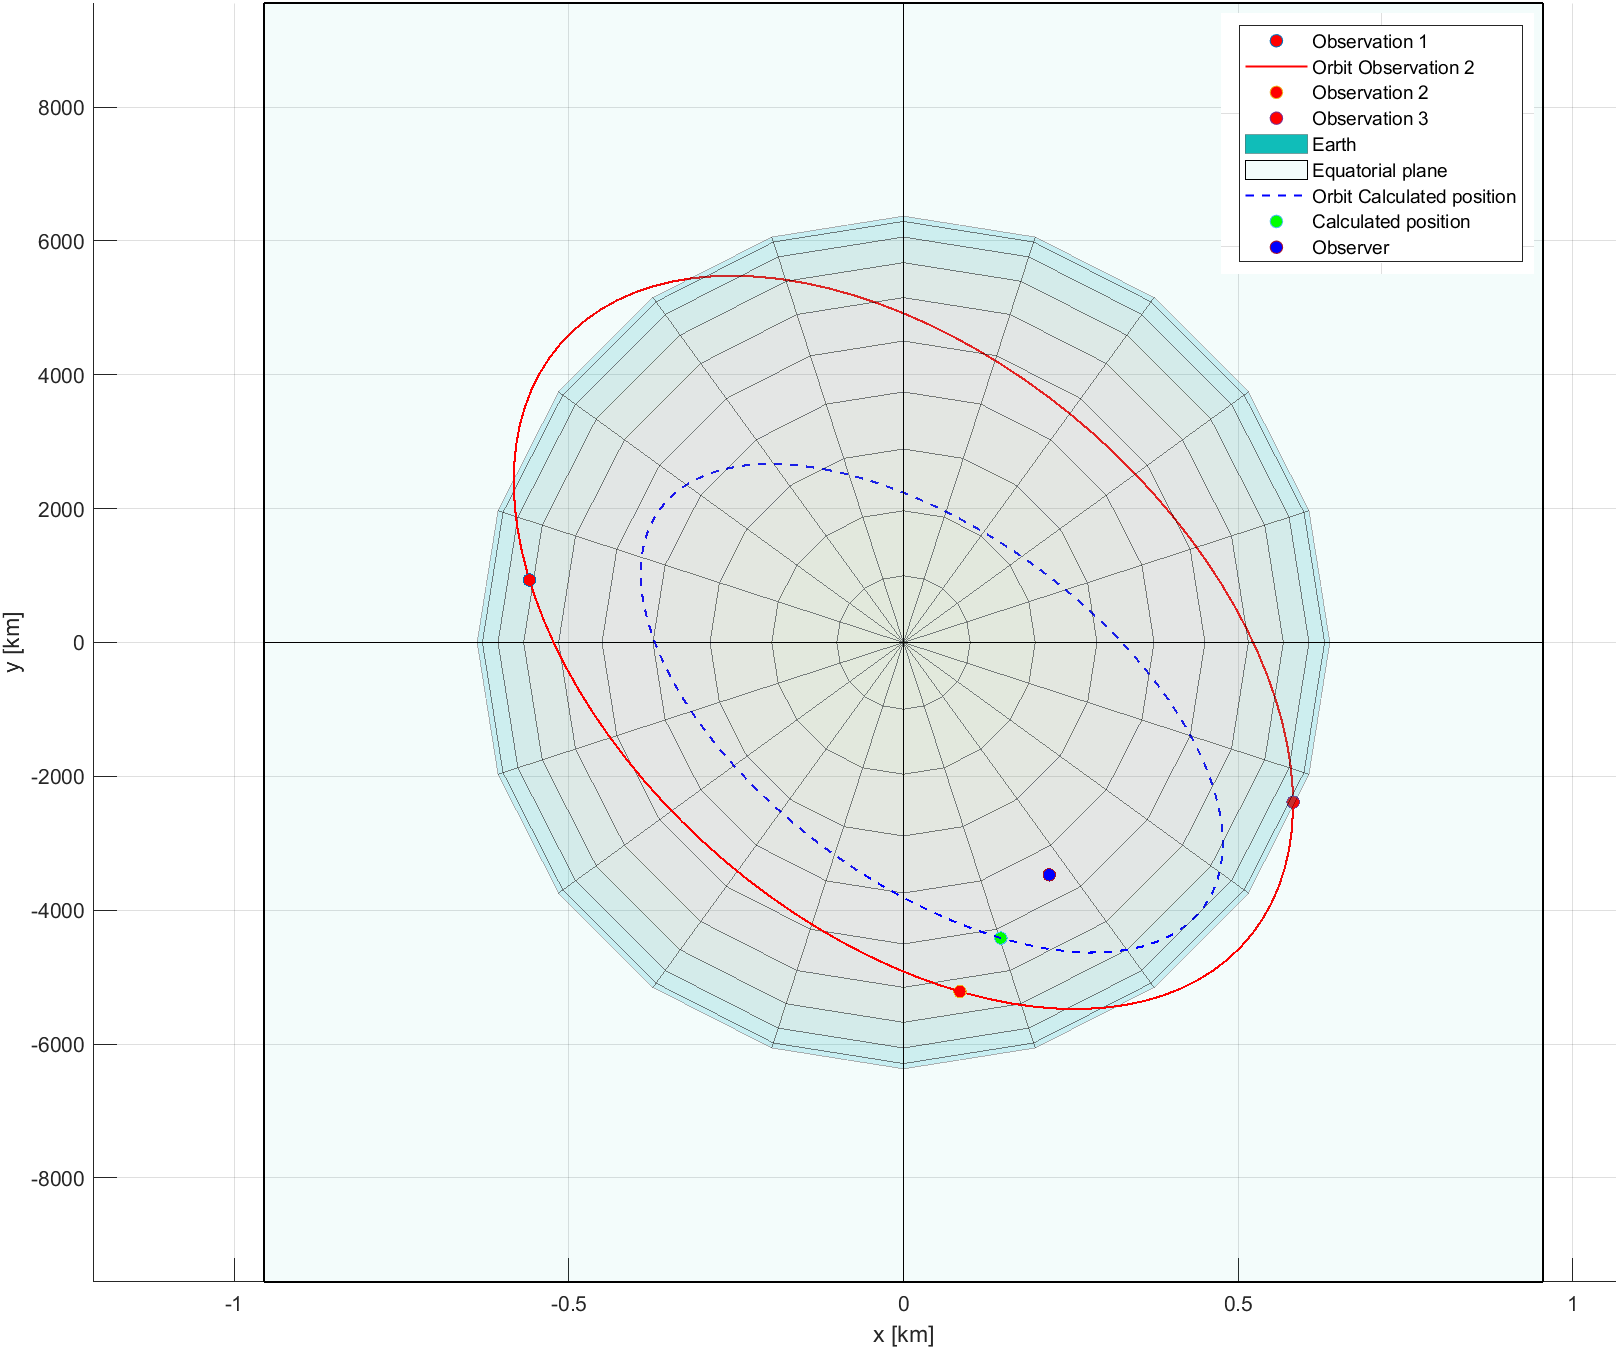
\includegraphics[width=\textwidth]{tex/img/anomaly82_rownikowa.png}
    \caption{Obserwacje hipotetyczne - rzut na płaszczyznę równikową}
    \label{fig:hipotetyczne-2}
    \end{figure}


\FloatBarrier
\subsection{Obserwacja rzeczywista}
 Do obserwacji wykorzystano program Stellarium. Interfejs aplikacji pokazuje Rys. \ref{fig:stellarium-interfejs}. Obserwatora umieszczono na współrzędnych 51\degree 23' 15" N, 18\degree 34' 10" E. Zaobserwowano przelot, który odbył się 19 grudnia 2022 między godziną 8:52 i 8:57 UTC. Czas wybrano z uwagi na zgodność daty z TLE i długi okres widoczności.
    \begin{figure}
    \centering
    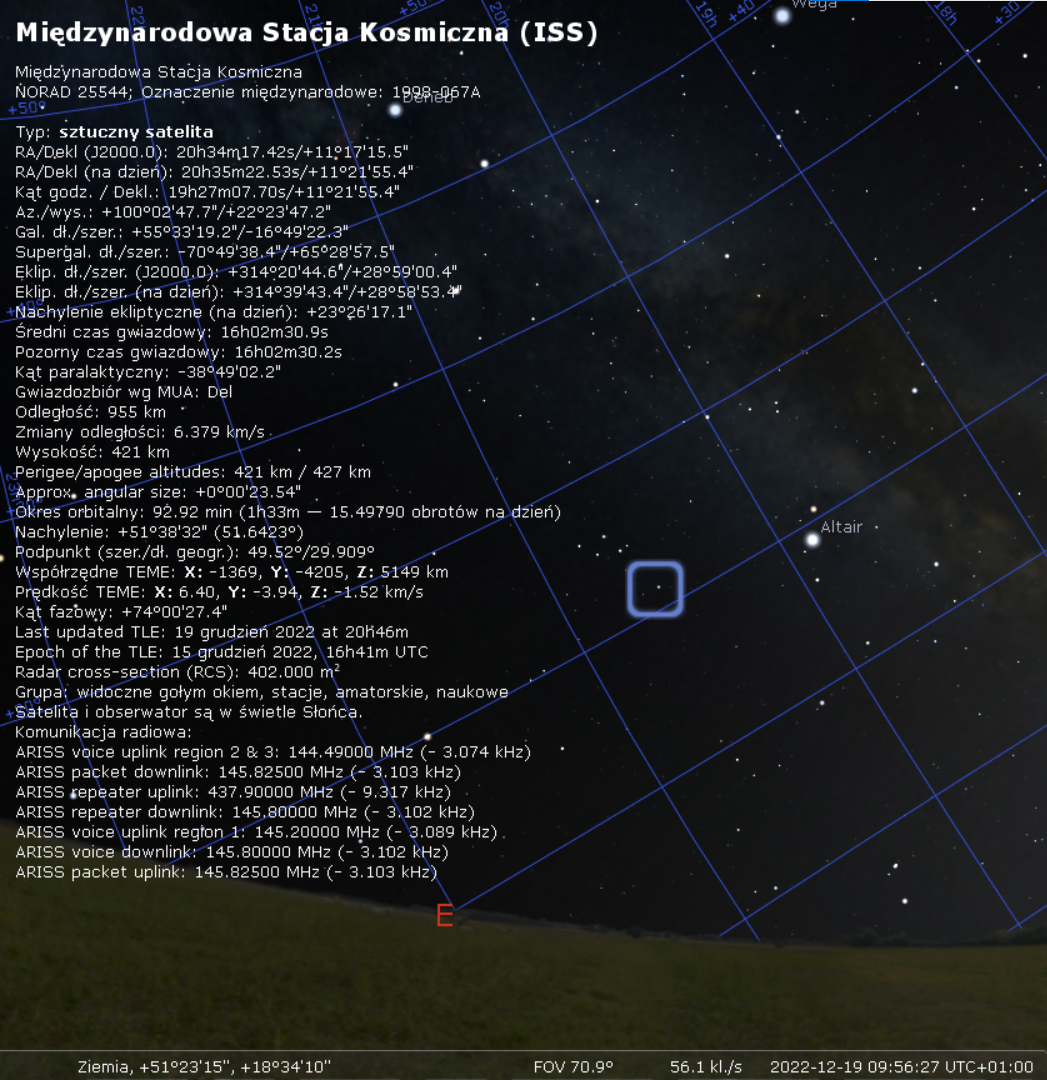
\includegraphics[width=\textwidth]{tex/img/ISSStellarium.png}
    \caption{Interfejs symulatora nocnego nieba Stellarium wykorzystanego do dokonania obserwacji}
    \label{fig:stellarium-interfejs}
    \end{figure}

    \subsubsection{Dane obserwacyjne}

    Czas obserwacji: 
        \begin{align*}
            t_1 &= 52'24" \\
            t_2 &= 54'26"  \\
            t_3 &= 56"35'
        \end{align*}
        
    Czas gwiazdowy obserwacji: 
        \begin{align*}
            \theta_1 &= 15\degree 28'27.1" \\
            \theta_2 &= 16\degree 00'29.8"  \\
            \theta_3 &= 16\degree 02'39.0"
        \end{align*}

    Wykorzystane pozycje [km]: 
   
            \begin{center}
              $\begin{bmatrix}
                R_{1x} & R_{1y} & R_{1z} \\
                R_{2x} & R_{2y} & R_{2z} \\
                R_{3x} & R_{3y} & R_{3z} 
            \end{bmatrix}
            =
            \begin{bmatrix}
                -2854 & -3102 & 5302 \\
                -2127 & -3692 & 5284 \\
                -1317 & -4237 & 5136
            \end{bmatrix}    $
        \end{center}

    \subsubsection{Wyniki}
    
    Pozycja wyznaczona przez program Stellarium pochodzi z bardziej zaawansowanego modelu, niż ten wykorzystywany do aproksymacji, co tłumaczy brak zgodności wyników. Mimo tego orbita została wyznaczone w przybliżeniu poprawnie, chociaż jest ona bardziej ekscentryczna. 

    \begin{table}[!h]  \centering
    \caption{Obserwacja rzeczywista - porównanie wyników}
    \label{tab:Stellarium-table}
    \begin{tabular} {| l | r | r | r |} \hline
        Parametr 1          & Wartość referencyjna  & Wartość wyznaczona  & Błąd \\ \hline\hline
        Moduł położenia w 2 pozycji     & 6788 km   & 6789         & 0.77 km\\ \hline
        Moduł prędkości w 2 pozycji     & 7.7 km/s     & 7.7 km/s     & 0.04 km/s\\ \hline
        Mimośród                        & 0.0004       & 0.0123       & 0.0119 \\ \hline
        Półoś wielka                    & 6794 km    & 6873 km        & 78 km \\ \hline
        Inklinacja                      & 51.64\degree & 51.63\degree & -0.018\degree \\ \hline
        Rektascensja węzła wstępującego & 138.9\degree & 139.2\degree & 0.23 \degree \\ \hline
        Argument perycentrum            & 174.7\degree & 97.6\degree  & -76.9 \\ \hline
        Anomalia prawdziwa              & 282\degree   & 356\degree   & 74 \\ \hline
    \end{tabular}
    \end{table}

    \begin{figure}[h]
    \centering
    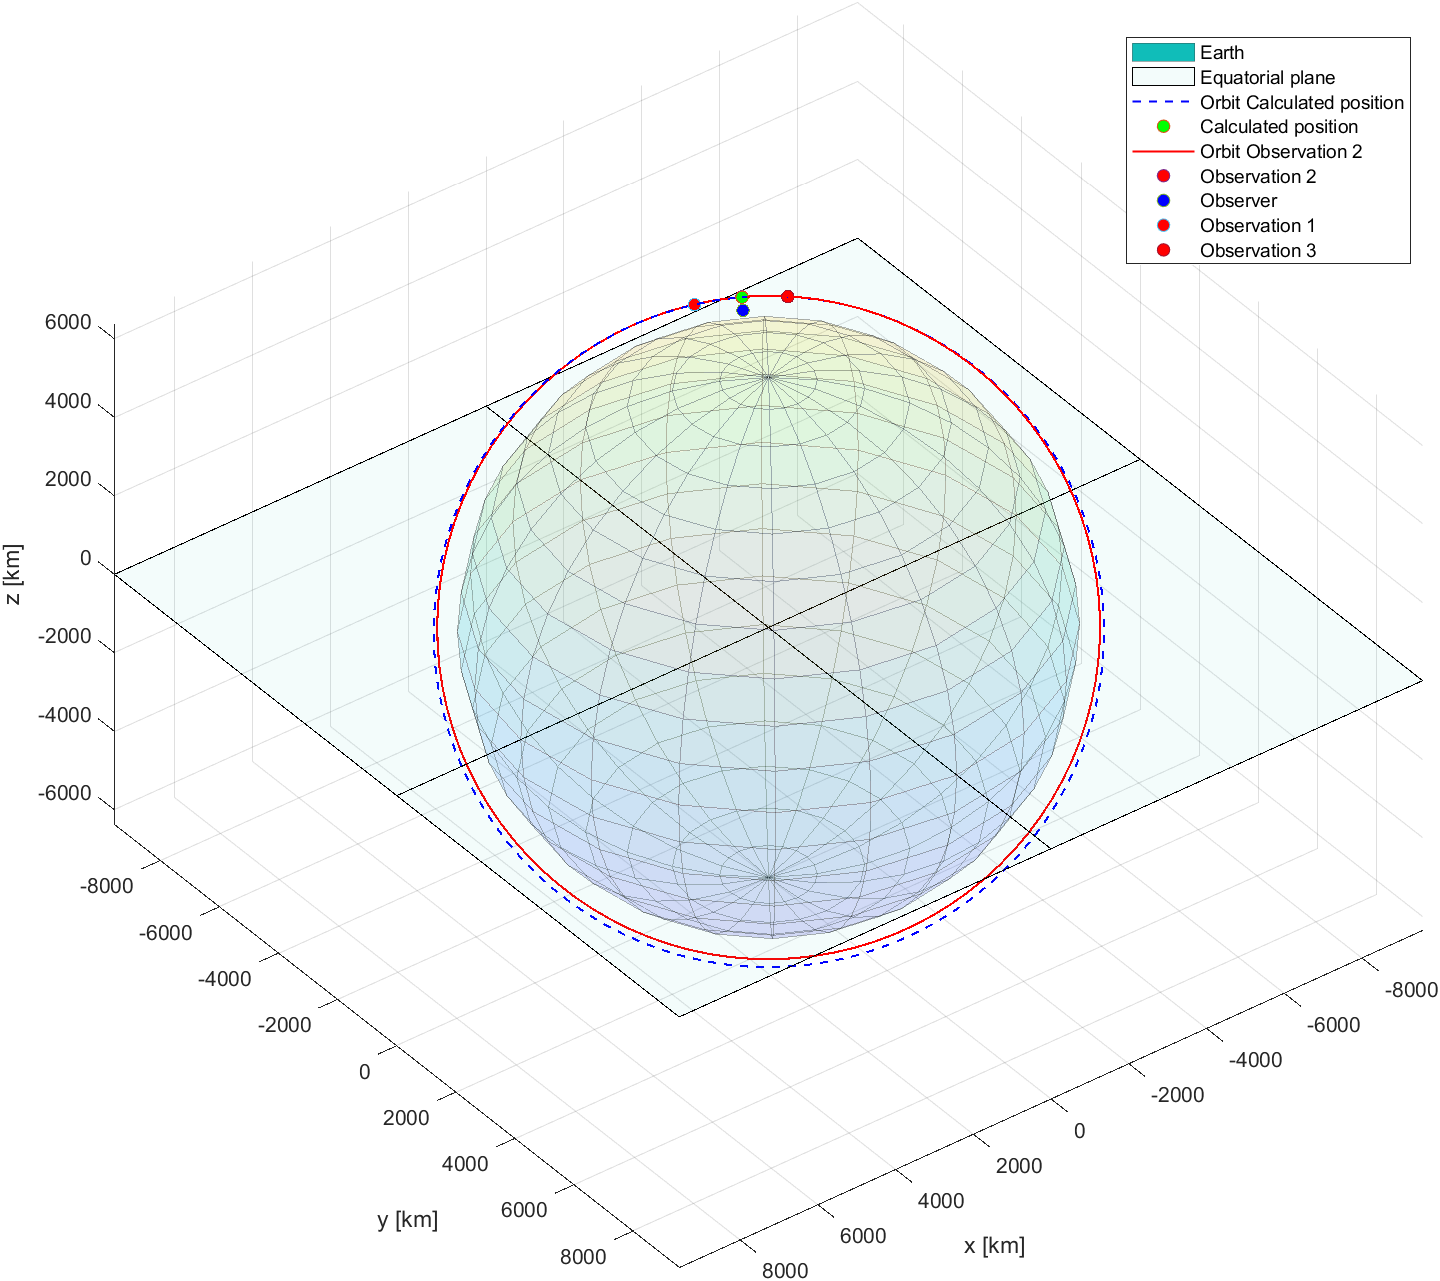
\includegraphics[width=\textwidth]{tex/img/StellariumFigure.png}
    \caption{Obserwacja na podstawie symulatora nieba}
    \label{fig:Stellarium-1}
    \end{figure}
    
    \begin{figure}[h]
    \centering
    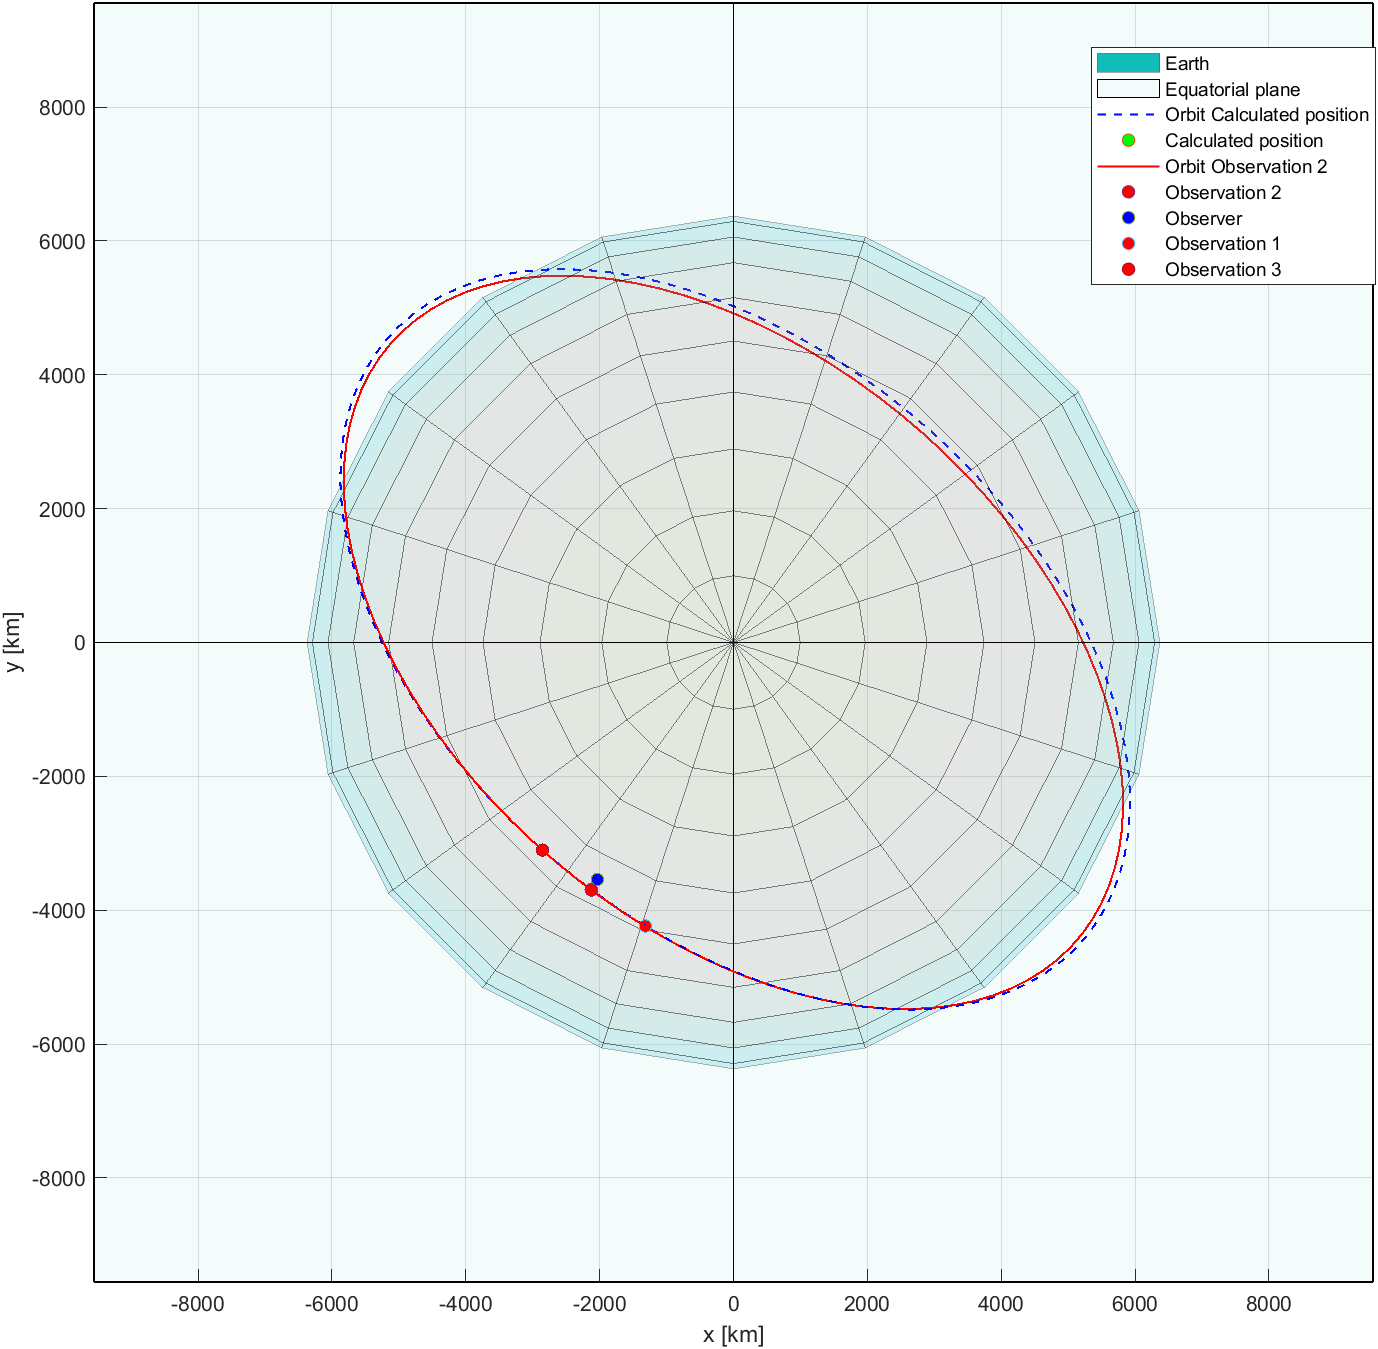
\includegraphics[width=\textwidth]{tex/img/StellariumFigure_rownikowa.png}
    \caption{Obserwacja na podstawie symulatora nieba - rzut na płaszczyznę równikową}
    \label{fig:Stellarium-2}
    \end{figure}
\FloatBarrier
\clearpage % Rozdziały zaczynamy od nowej strony.
\section{Podsumowanie}

W ramach przedstawionego zagadnienia sprawdzono stosowalność metody Gaussa do wstępnego wyznaczania orbit obiektów kosmicznych na podstawie obserwacji naziemnych. W tym celu zaimplementowano metodę w formie programu oraz przygotowano zbiory danych walidacyjnych. Metoda wykorzystuje założenie, że czasy między kolejnymi pomiarami są niewielkie względem okresu orbity i dla przypadków zgodnych z założeniami jest skuteczna. Jeśli międzyczasy są zbyt małe, to nawet drobne błędy w obserwacji mogą spowodować duże rozbieżności w obliczonej orbicie. Wykonanie pomiarów w trakcie jednego przebiegu orbity - podczas wschodu, zenitu i zachodu obiektu pozwala uzyskać optymalne wyniki, jednocześnie zachowując pewność, że obserwowany jest ten sam obiekt. 


% Umożliwia to również łatwą migrację do nowej wersji szablonu:
 % zazwyczaj wystarczy podmienić plik src/wut-thesis.cls

 % Można też pisać rozdziały w jednym pliku.

%--------------------------------------------
% Literatura
%--------------------------------------------
\cleardoublepage % Zaczynamy od nieparzystej strony
\printbibliography

%--------------------------------------------
% Spisy (opcjonalne)
%--------------------------------------------
\newpage
\pagestyle{plain}

\listoffigurestoc     % Spis rysunków.
\vspace{1cm}          % vertical space
\listoftablestoc      % Spis tabel.


\section*{Załączniki}

\subsection{Warianty symulacji}

    \lstinputlisting{tex/code/startCustomData.m} 
    \lstinputlisting{tex/code/startStellariumData.m} 

\subsection{Algorytm Gaussa}
    \lstinputlisting{tex/code/observation2state.m} 
    \lstinputlisting{tex/code/refineStateMeasurement.m} 
    \lstinputlisting{tex/code/state2OrbitalElements.m} 

\subsection{Uniwersalne równanie Keplera}
    \lstinputlisting{tex/code/solveUniversalKepler.m} 
    \lstinputlisting{tex/code/StumpffC.m} 
    \lstinputlisting{tex/code/StumpffC.m} 
    
\subsection{Konwersja danych}
    \lstinputlisting{tex/code/findStationPosition.m} 
    \lstinputlisting{tex/code/angles2directionCosines.m} 
    \lstinputlisting{tex/code/convertOE.m} 
       
\subsection{Symulacja ISS}
    \lstinputlisting{tex/code/ISSClass.m}   

\subsection{Wyświetlanie wyników}
    \lstinputlisting{tex/code/displayData.m} 
    \lstinputlisting{tex/code/plotEarth.m} 
    \lstinputlisting{tex/code/plotFromOE.m} 

 

% Używając powyższych spisów jako szablonu,
% możesz tu dodać swój własny wykaz bądź listę,
% np. spis algorytmów.

\end{document} % Dobranoc.
